\documentclass{sig-alternate-2013}%{acm_proc_article-sp}%{sig-alternate}%
%\documentclass{vldb}
%\documentclass[10pt,conference,letterpaper]{IEEEtran}
\usepackage{amsmath}
\usepackage{multicol}
%\usepackage{algorithm}
\usepackage{algorithm}
%\usepackage[ruled,vlined]{algorithm}
\usepackage{algorithmic}
%\usepackage{hyperref}%[colorlinks, citecolor=blue, hyperindex]
\usepackage{graphicx,subfigure}
\usepackage{url}
\usepackage{color}
%\usepackage{algorithm2e}
%\usepackage{subfigure}
\graphicspath{{figures/}}
\newcommand{\KZ}[1]{\textcolor{blue}{[KZ: #1]}}
\renewcommand{\sim}[2]{\textsc{sim}(\textit{#1}, \textit{#2})}
\newcommand{\pair}[2]{$\langle #1, #2 \rangle$}
\newcommand{\LP}[1]{\textcolor{red}{[LP: #1]}}
\newcommand{\secref}[1]{Section \ref{#1}}
\newcommand{\figref}[1]{Figure \ref{#1}}
\newcommand{\eqnref}[1]{Eq. (\ref{#1})}
\newcommand{\argmin}{\operatornamewithlimits{argmin}}
\newcommand{\argmax}{\operatornamewithlimits{argmax}}
%\newcommand{\exref}[1]{Example \ref{#1}}

%\usepackage{caption}
\newfont{\mycrnotice}{ptmr8t at 7pt}
\newfont{\myconfname}{ptmri8t at 7pt}
\let\crnotice\mycrnotice%
\let\confname\myconfname%

\permission{Permission to make digital or hard copies of all or part of this work for personal or classroom use is granted without fee provided that copies are not made or distributed for profit or commercial advantage and that copies bear this notice and the full citation on the first page. Copyrights for components of this work owned by others than ACM must be honored. Abstracting with credit is permitted. To copy otherwise, or republish, to post on servers or to redistribute to lists, requires prior specific permission and/or a fee. Request permissions from Permissions@acm.org.
}
\conferenceinfo{CIKM'13,}{October 27 - November 01 2013, San Francisco, CA, USA.}
\copyrightetc{Copyright 2013 ACM \the\acmcopyr}
\crdata{978-1-4503-2263-8/13/10\ ...\$15.00.\\
http://dx.doi.org/10.1145/2505515.2505567}

\clubpenalty=10000
\widowpenalty = 10000

\begin{document}
\title{Computing Term Similarity by Large Probabilistic isA Knowledge}
%\author{%
%% author names are typeset in 11pt, which is the default size in the author block
%{Peipei Li{\small $~^{\#*1}$}, Haixun Wang{\small $~^{*2}$}, Kenny Q. Zhu{\small $~^{\dag3}$}, Zhongyuan Wang{\small $~^{*2}$}, Xindong Wu{\small $~^{\ddag4}$} } %
%% add some space between author names and affils
%\vspace{1.6mm}\\
%\fontsize{10}{10}\selectfont\itshape
%$~^{\#}$Hefei University of Technology\\
%%Hefei, China\\
%\fontsize{9}{9}\selectfont\ttfamily\upshape
%$~^{1}$v-pli@microsoft.com\\
%% add some space between email and affil
%\fontsize{10}{10}\selectfont\rmfamily\itshape
%$~^{*}$Microsoft Research Asia\\
%\fontsize{9}{9}\selectfont\ttfamily\upshape
%$~^{2}$\{haixunw,zhy.wang\}@microsoft.com\\
%\fontsize{10}{10}\selectfont\rmfamily\itshape
%$~^{\dag}$Shanghai Jiao Tong University\\
%%, Shanghai, China\\
%\fontsize{9}{9}\selectfont\ttfamily\upshape
%$~^{3}$kzhu@cs.sjtu.edu.cn\\
%\fontsize{10}{10}\selectfont\rmfamily\itshape
%$~^{\ddag}$University of Vermont\\
%\fontsize{9}{9}\selectfont\ttfamily\upshape
%$~^{4}$xwu@uvm.edu }
\numberofauthors{5} %  in this sample file, there are a *total*
% of EIGHT authors. SIX appear on the 'first-page' (for formatting
% reasons) and the remaining two appear in the \additionalauthors section.
%
\author{
% You can go ahead and credit any number of authors here,
% e.g. one 'row of three' or two rows (consisting of one row of three
% and a second row of one, two or three).
%
% The command \alignauthor (no curly braces needed) should
% precede each author name, affiliation/snail-mail address and
% e-mail address. Additionally, tag each line of
% affiliation/address with \affaddr, and tag the
% e-mail address with \email.
%
% 1st. author
\alignauthor
Peipei Li\titlenote{Peipei Li was a student intern in Microsoft Research Asia when the paper was
developed.}\\
       \affaddr{Hefei University of Technology}\\
       \affaddr{Hefei, China, 230009}\\
       \email{peipeili\_hfut@163.com}
% 2nd. author
\alignauthor
Haixun Wang\\%\titlenote{The secretary disavows any knowledge of this author's actions.}\\
       \affaddr{Microsoft Research Asia}\\
       \affaddr{Beijing, China, 100080}\\
       \email{haixunw@microsoft.com}
% 3rd. author
\alignauthor
Kenny Q. Zhu\\%\titlenote{This author is the one who did all the really hard work.}\\
       \affaddr{Shanghai Jiao Tong University}\\
       \affaddr{Shanghai, China}\\
       \email{kzhu@cs.sjtu.edu.cn}
\and  % use '\and' if you need 'another row' of author names
% 4th. author
\alignauthor Zhongyuan Wang\\
       \affaddr{Renmin University of China}\\
       \affaddr{Beijing, China, 100872}\\
       \affaddr{Microsoft Research Asia}\\
       \affaddr{Beijing, China, 100080}\\
       \email{zhy.wang@microsoft.com}
% 5th. author
\alignauthor Xindong Wu\\
       \affaddr{University of Vermont}\\
       \affaddr{Vermont, U.S.A., 05405}\\
       \email{xwu@uvm.edu}
}
% There's nothing stopping you putting the seventh, eighth, etc.
% author on the opening page (as the 'third row') but we ask,
% for aesthetic reasons that you place these 'additional authors'
% in the \additional authors block, viz.
%\additionalauthors{Additional authors: John Smith (The Th{\o}rv{\"a}ld Group,
%email: {\texttt{jsmith@affiliation.org}}) and Julius P.~Kumquat
%(The Kumquat Consortium, email: {\texttt{jpkumquat@consortium.net}}).}
%\date{30 July 1999}
% Just remember to make sure that the TOTAL number of authors
% is the number that will appear on the first page PLUS the
% number that will appear in the \additionalauthors section.
\maketitle
\begin{abstract}
  Computing semantic similarity between two terms is essential for a
  variety of text analytics and understanding applications.
%  Currently, there are two main approaches for this task,
%  namely the knowledge based and the corpus based approaches.
 However, existing approaches are more suitable for
  semantic similarity between words rather than the more general multi-word
  expressions (MWEs), and they do not scale very well.
  % and scalability issues from manual tagging as well
  %as corpora dependency and availability also limit their applicability.
  %Contrary to these existing techniques,
  Therefore, we propose a lightweight and effective approach
  for semantic similarity using a large scale semantic network
  automatically acquired from billions of web documents.
  %The semantic
  %network consists of millions of concepts, which explicitly model the
  %context of semantic relationships.
  Given two terms, we map them into the concept space, and compare
  their similarity there. Furthermore, we introduce a clustering approach to
  orthogonalize the concept space in order to improve the accuracy of
  the similarity measure. %  identify potential senses of terms instead
  % of manually tagging, and then compare the term's sense based
  % contexts to get the semantic similarity between terms.
  Extensive studies demonstrate that our approach can accurately
  compute the semantic similarity between terms with MWEs and ambiguity,
  and significantly outperforms 12 competing methods.
%  Comparison with 12 similarity methods
%  shows that our approach on average outperforms the best existing
%  method by 17.6\% on word pairs and 34.6\% on MWEs
%  in terms of {\color{red}{Pearson Correlation Coefficient}} in similarity, and reaches an average of 0.77
%  on word pairs and 0.67 on MWE pairs by the Pearson Correlation Coefficient.
%
%  The pearson correlation coefficient is
%  improved by the range of [0.07, 0.41] \LP{The difference of PCC between our RCP approach with the best one of other competing methods is 0.056, 0.03, 0.105 respectively on three data sets while the PCC in RCP is 0.921, 0.725, 0.735 respectively on three data sets. The improvement percent is 0.065, 0.043 and 0.167.}compared to the state-of-the-art approaches
%  for the semantic similarity measurement between terms.
%  Meanwhile, our approach is very efficient and can be applied on computing
%  semantic similarity in a large scale.
\end{abstract}

% , and knolnumber
  % of conceptualization In order Meanwhile, in a massive corpus, a
  % substantial fraction of extractions appear infrequently. It is hence
  % a challenge for traditional information extraction techniques to
  % assess these large scale sparse extractions. Motivated by this
  % challenge, this paper shows how to assess the correctness of sparse
  % extractions by utilizing the semantic context-based assessment
  % approach. In our proposed method, we adopt three different semantic
  % contexts. Firstly, we use the conceptualization method to get a set
  % of representative concepts from the sentences as the
  % context. Secondly, we extract the attributes as the
  % context. Thirdly, we collects the isA concepts as the context. In
  % terms of these semantic contexts, we implement a similarity
  % evaluation to rank extractions by the likelihood that they are
  % correct. Lastly, we apply our approach into the Hearst pattern
  % database of Probase, which contains 2425558 concepts and 15805500
  % extractions extracted using Hearst patterns from 1.68 billion web
  % pages and two years' worth of Microsoft Bing's search
  % log.


% A category with the (minimum) three required fields
%\category{H.4}{Information Systems Applications}{Miscellaneous}
%A category including the fourth, optional field follows...
%\category{D.2.8}{Software Engineering}{Metrics}[complexity measures, performance measures]

%\terms{Theory}

% A category with the (minimum) three required fields
\category{H.3}{INFORMATION STORAGE AND RETRIEVAL}{Miscellaneous}
%A category including the fourth, optional field follows...
\category{I.2}{Computing Methodologies}{ARTIFICIAL INTELLIGENCE}[Knowledge Representation Formalisms and Methods]

%\terms{Algorithms,Measurement}

\keywords{Term Similarity; Multi-word Expression; Clustering; Semantic Network} % NOT required for Proceedings

%\keywords{ACM proceedings, \LaTeX, text tagging} % NOT required for Proceedings
\section{Introduction}
%\KZ{What's the definition of term? What is term similarity? Explain briefly the diff between
%similarity and relatedness. Why is term similarity important?}
%\KZ{One problem is that we don't handle verbs or adjectives. We
%need to point this out either in the title or somewhere here.}

Measuring semantic similarity between terms is a fundamental problem
in lexical semantics \cite{Budanitsky:2006} and it finds many
applications in web and document search \cite{WangLWZ12:Concept}, question and answer systems,
and other text analytics and text understanding scenarios.  By {\em
  terms}, we mean either single words or multi-word expressions
(MWEs).
%{\color{red}in this paper, we refer terms as the collective
%concepts and entities}.
We say two terms are semantically similar, if their
meanings are close, or the concept or object that they represent share many common attributes.  For example, ``emerging markets'' and
``developing countries'' are similar because their semantic contents (the subset of countries) are very similar. Another example, ``Google'' and
``Microsoft'' are similar because they are both software companies. %  and
% as a software company, they share a number of commonalities.
However, ``car'' and ``journey'' are not semantically similar but {\it related} because ``car'' is a transport means for
  the activity ``journey''. Specifically, semantic
similarity is defined by some measure of {\em distance} between two terms on an isA taxonomy.
%which organizes terms by {\em synonymy} and {\em hypernumy} relations.
% Such distance can be either a naive metric of number of distinct edges
% (hops) between two nodes on the taxonomy graph, or more sophisticated
% statistical measures.
It is clear that ``car'' and ``journey'' are quite far away from each other in an isA taxonomy from WordNet as shown in Figure~\ref{fig:tree}.
Semantic similarity is a more specific relationship and is much harder to model than {\em relatedness} (which can be modeled by term
co-occurrence).
% In this paper, we are concerned
% with the efficient computation of semantic similarity between two
% terms.
\begin{figure}[th]
 \centerline{
 \includegraphics[width=0.5\textwidth]{car-journey.eps}}
\caption{A fragment from WordNet showing semantic distance between ``car'' and ``journey''}
\label{fig:tree}
\end{figure}
%\KZ{Include a graph cut from wordNet that shows the distance between
%car and journey.}

%Semantic similarity is different from semantic relatedness.
% Contrary to the semantic relatedness relying on the more general relationships (e.g., part-of and the co-occurrence), semantic similarity relies on the degree of taxonomic
%likeness between concepts considering relationships such as hyponymy and hyperonymy, but most of the semantic similarity measurement methods can be adapted and generalized to deal with semantic relatedness.
%We can adapt and generalize the semantic similarity measurement methods to deal with semantic relatedness, but we cannot adapt the semantic relatedness measurement methods to deal with semantic similarity. For example, \emph{journey} and \emph{car} has a high semantic relatedness score due to the higher co-occurrences in the corpus, while its semantic similarity should be lower because they belong to the different concepts.


%\KZ{Briefly state the existing approaches. Classify them into two categories. State why they don't work for some
%examples. Use concrete examples (challenge 1-3) from the slides to
%illustrate the challenges.}
% Computing the semantic similarity between two terms is tantamount to
% computing the similarity between their {\em contexts}.
Recent work on term similarity can be roughly classified into two main categories: {\em knowledge based} and {\em corpus based}. Knowledge based
approaches rely on handcrafted resources such as thesauri, taxonomies or encyclopedias, as the context of comparison.  Most work in this space
\cite{Rada:1989, Resnik:1995, Agirre:2010} depends on the semantic isA relations in WordNet \cite{Miller1995} which is a manually curated
lexicon and taxonomy. Corpus based approaches work by extracting the contexts of the terms from large corpora and then inducing the
distributional properties of {\em words} or {\em
  n-grams}.
%{\color{red}(It also include the term co-occurrence based method)}.
Corpus can be anything from web pages, web
search snippets to other text repositories.
%For example, Google distance \cite{Cilibrasi:Google} is
%derived from the number of hits returned by the Google search engine.
%Other corpus-based measures rely on the
%content of search results or search snippets.

One significant challenge faced by the knowledge-based methods is the
limited coverage of taxonomies such as WordNet (with 155,287 words
at last count).
%Through two decades of development, the most recent release
%of WordNet (version 3.0) contains
%155,287 words organized in 117,659 synsets and 206,941 word-sense pairs.
It does not cover many proper nouns (e.g., ``Microsoft''
or ``Google''), or very popular senses (e.g., Apple the company or
Jaguar the car make). Another major restriction of WordNet is that it
primarily covers single words with only a handful of phrases or
multi-word expressions.  For example, it does not know ``General
Electric'' or ``emerging markets''.
%Thus, it is impossible for these
%WordNet-based methods to correctly compute the semantic similarity
%which involves these unknown terms or terms with unknown senses.
Consequently, the similarity between ``General Electric'' and ``GE''
is completely ignored.
%they are exactly the same thing.
%With today's fast changing world, it is just not possible for manually
%curated lexical databases like WordNet to keep up with the pace of the
%creation of new words and phrases in human languages.
%
%Meanwhile, new words are constantly being
%created on the Web as well as new senses are assigned to existing words,
%it is also costly for manually maintaining existing thesauri like
%WordNet to capture these new words and senses if not impossible.

Corpus-based approaches also face several serious limitations.
First, such measures are biased because of the indexing and 
ranking mechanisms used in search engines. 
% Unfortunately, these mechanisms are often ``commercial
% secrets'' and are opaque to outsiders.
For example when querying the term ``date''
%\footnote{sense 1: day of the month; ...; sense 8: sweet edible fruit of the
%date palm with a single long woody seed.}
or ``range''
%\footnote{sense 1: scope; ...; sense 9: stove, kitchen stove. Senses of
%``date'' and ``range'' mentioned above are annotated in WordNet.}
on Google, none of the first 100 results has anything to do with
fruits (a sense for date) or cooking stoves (a sense for range),
because these are rare senses of the two terms.
%and are considered not ``relevant'' by Google.
With such search results, it is not surprising that a corpus-based
method would think ``asian pear'' and ``date'' share very little commonality.
%and ``food processor'' and ``range'' are very different, too.
Second, some search-result oriented similarity methods require
interaction with the search engine which has high communication overhead
and high index costs, and are not suitable for online applications.
%Hence they are not suitable for online applications which require fast
%response time.
%For the second distributional context based approach, in order to
%extend the data coverage, it adopts the search snippets or web documents
%as the corpus. This indicates this approach heavily depends on the
%search engine's ranking algorithm.
Third, statistical distribution based on words or n-grams in the
context ignores the fact that i) the semantic units can be MWEs and not
words, let alone n-grams; and ii) many words or phrases are ambiguous
in meaning. %e.g., ``apple'' can be both a fruit and a company.
%Consequently, distribution thus computed may not truly represent the
%semantic landscape of the contexts. To fix this problem, some methods
%in this category resorted to manual labeling of senses in a machine
%learning approach \cite{Bollegala:2007, Bollegala:Supervised} which is
%tedious and time-consuming.
Finally, corpus-based methods focus on
surrounding context of a term or the co-occurrence of two terms within
a neighborhood, both of which are more suitable to the calculation of
semantic relatedness rather than similarity.  Under this approach,
``car'' and ``journey'' would have high semantic relatedness because
they co-occur very frequently on web texts.
%when in fact they are {\em  not} similar because
%$Apple$ is a company and $iPad$ is a product by the company.

% \begin{figure}[t]
% %\makeatletter\def\@captype{figure}\makeatother
%  \centerline{
%  \includegraphics[width=0.5\textwidth]{Correlation-on-MC-r.eps}}
% \caption{Pearson correlation coefficient in different approaches} \label{fig:Correlation-on-MC}
% \end{figure}
%
% \begin{table}[!h]
% \centering
% \caption{Concept lists of a pairwise term Microsoft and Apple}% (extracted using Hearst patterns)}
% \label{tab:microsoft-apple}
% \begin{tabular}{|l|c|l|c|}\hline
% concepts of Microsoft & weight & concepts of Apple & weight\\\hline
% company   &0.4239 &fruit  &0.2952\\
% u.s. company  &0.0349 &company    &0.1362\\
% large company &0.0321 &seasonal fruit &0.0826\\
% client    &0.0256 &food   &0.0612\\
% organization  &0.0217 &fresh fruit    &0.0389\\
% software giant    &0.0217 &fruit tree &0.0223\\
% international company &0.0207 &brand  &0.0216\\
% provider  &0.0184 &crop   &0.0147\\
% industry leader   &0.0184 &flavor &0.0121\\
% technology company    &0.0145 &manufacturer   &0.0100\\
% software company  &0.0141 &tree   &0.0083\\
% big company   &0.0125 &competitor &0.0077\\
% giant &0.0123 &product    &0.0067\\
% player    &0.0112 &juice  &0.0067\\
% software vendor   &0.0095 &fruit juice    &0.0065\\
% competitor    &0.0086 &snack  &0.0054\\
% partner   &0.0082 &healthy snack  &0.0052\\
% manufacturer  &0.0071 &dried fruit    &0.0051\\
% industry giant    &0.0068 &large company  &0.0048\\
% big player    &0.0063 &tree fruit &0.0048\\
% \hline
% \end{tabular}
% \end{table}
%
% \begin{table}[!h]
% \centering
% \caption{Concept clusters of a pairwise term Microsoft and Apple}% (extracted using Hearst patterns)}
% \label{tab:microsoft-apple-clusters}
% \begin{tabular}{|p{2pt}|l|c|p{2pt}|l|c|}\hline
%  & concepts &  &  & concepts & \\
% id & of Microsoft & weight & id & of Apple & weight\\\hline
% 1 &company    &0.3738 &1  &fruit  &0.2952\\
% 1 &u.s. company   &0.0349 &1  &seasonal fruit &0.0826\\
% 1 &client &0.0256 &1  &tree fruit &0.0048\\
% 1 &large company  &0.0227 &1  &fresh fruit    &0.0389\\
% 1 &software giant &0.0217 &1  &juice  &0.0067\\
%   &international-&    &   &   &\\
% 1 &company    &0.0207 &1  &fruit juice    &0.0065\\
%   &technology-    &   &   &   &\\
% 1 &company    &0.0145 &1  &dried fruit    &0.0051\\
% 1 &software company   &0.0141 &2  &company    &0.1239\\
% 1 &big company    &0.0125 &2  &manufacturer   &0.0100\\
% 1 &giant  &0.0123 &2  &competitor &0.0077\\
% 1 &player &0.0112 &2  &large company  &0.0048\\
% 1 &software vendor    &0.0095 &3  &food   &0.0612\\
% 1 &competitor &0.0086 &3  &snack  &0.0054\\
% 1 &partner    &0.0082 &3  &healthy snack  &0.0052\\
% 1 &manufacturer   &0.0071 &4  &fruit tree &0.0223\\
% 1 &industry giant &0.0068 &4  &tree   &0.0083\\
% 1 &big player &0.0063 &5  &brand  &0.0216\\
% 2 &organization   &0.0217 &6  &crop   &0.0147\\
% 3 &provider   &0.0184 &7  &flavor &0.0121\\
% 4 &industry leader    &0.0184 &8  &product    &0.0067\\
% \hline
% \end{tabular}
% \end{table}

%\KZ{Briefly give the problem statement. Don't talk about the specific challenges below which are details of
%the approach. But briefly mention what is our approach: 1) judge the types of the terms; 2) collect the context
%of the terms by clustering the their sense; 3) compute the similarity.
%Stress that our key difference is 1) the use of a large semantic network extracted from
%very big data which shows  the power of universal knowledge from the web; 2) our approach is very fast
%compared to previous approach because... You can show the similarity result from our system on the few
%difficult examples in the previous paragraph. No need to show detailed tables or figures. Just let the reader
%get an idea of what you can achieve and how accurate your approach is!}

In this paper, we propose a light-weight but effective framework for
computing semantic similarity %(a number between 0 and 1)
between a pair of terms using a large scale, general purpose isA
network obtained from a web corpus. It belongs to the knowledge-based method.
% The framework computes similarity in three simple steps:
% \begin{enumerate}
% \item typecheck the input terms into either an {\em entity} or a {\em concept};
% \item represent the semantic contexts of each term according to its type and its
% position in the isA semantic network and disambiguate the senses of the input
% terms by clustering the super-concepts or the subsumed entities within the
% network;
% \item computing similarity between the probability distribution of the two contexts
% using a max-max similarity function.
% \end{enumerate}
% With this novel approach, we are able to efficiently compute the semantic
% similarity between almost any MWEs. We focus on noun-based terms in this paper
% though the framework can be easily extended to verbs and adjectives as well.
Below is a small sample of results:

\begin{itemize}
\item High similarity (synonyms): \pair{general~ electric}{ge}
%  Synonyms that refer to the same entity should have the highest
%  similarity score.
\item High similarity (ambiguous terms): \pair{microsoft}{apple},
  \pair{orange}{red}
%  \sim{asian pear}{date}  =  0.7111 \\
%  Words such as ``apple'' and ``orange'' have multiple
%  senses. However, when people compare ``apple'' with ``microsoft'',
%  they consider ``apple'' in the sense of a company rather than a
%  fruit, and when they compare ``orange'' and ``red'', they consider
%  ``orange'' as a color rather than a fruit. Thus, disambiguation
%  needs to be performed by default in similarity comparison.

\item Low similarity (though share same hypernyms in WordNet):
\pair{music}{lunch}, \pair{banana}{beef}
%  These pairs of terms are not similar. However, in an isA network,
%  ``music'' and ``lunch'' may both belong to concepts such as
%  ``activity'', and ``banana'' and ``beef'' may both belong to concepts
%  such as ``food''. We may use their distances in a handcrafted
%  taxonomy to measure similarity, but handcrafted taxonomies have low
%  coverage, while distances in large scale, data driven semantic
%  networks are not easy to measure.

\item Low similarity (related but not similar): \pair{apple}{ipad}, \pair{car}{journey}
%  We need to differentiate similarity from relatedness. Here,
%  ``apple'' and ``ipad'', ``car'' and ``journey'' are related, but
%  they are not similar. {\color{red} This is because ``ipad'' is an electronic product of the company ``apple'' while ``car'' is a traffic tool for
%  the activity ``journey'', however, they belong to the different concepts or far away on an isA taxonomy.}
%
\end{itemize}

% \begin{eqnarray*}
% %\sim{General Electric}{GE} &=& 0.9875 \\
% \sim{General Electric}{GE} &=& 1.0\\
% \sim{Microsoft}{Apple} &=& 0.994 \\
% \sim{food processor}{range} & = & 0.6894 \\
% \sim{asian pear}{date} & = & 0.7111 \\
% \sim{apple}{ipad} &=& 0.0167 \\
% \sim{car}{journey} &=& 0.0001
% \end{eqnarray*}

%\begin{itemize}
%\item Large coverage;
%\item More meaningful similarity (e.g., apple and Microsoft);
%\item Lightweight
%\end{itemize}


%We introduce a scalable and effective approach for measuring
%the semantic similarity between terms in this paper.
The main contributions of this paper are:
\begin{itemize}
\item {\em Our approach has better coverage.}
The semantic network behind this approach is one order of magnitude larger
than WordNet in terms of the number of hypern-ym-hyponym relations.
%Unlike existing methods based on WordNet which only measure the similarity between limited number of words,
Our approach computes similarity between almost any two
known noun-based MWEs.
%This is because the knowledge source behind this approach
%is harnessed from billions of web documents.
%millions of terms, and then we compare the
%similarity between their contexts. It could be used to calculate
%semantic similarity between named entities, etc, which are not listed
%in WordNet or other manually compiled thesauri.

\item {\em Our approach produces more meaningful similarity.}
Unlike corpus-based methods which can confuse similarity with relatedness,
this approach calculates similarity by relations induced from an isA semantic
network. It also seeks to disambiguate terms
% with multiple meanings before calculating similarity
and thus excludes noises from irrelevant senses from
the probability distributions.
%As a result, the similarity results are more relevant and reliable.
%We introduce the concept clustering approach on the collected contexts
%given the term to identify its potential senses automatically,
%and then we utilize the term's sense based similarity evaluation
%method to improve the semantic similarity between terms especially
%for ambiguous terms with skewed data distributions of contexts.
%Thus, we can get more meaningful similarity between terms compared
%to the existing methods for semantic similarity.

\item {\em Our approach is lightweight.}  The most expensive
  clustering algorithm is performed offline.
  The remaining similarity function can be efficiently
  computed online. On average, it takes merely 65 milliseconds to
  compute the similarity for a pair of terms.
\end{itemize}

%\subsection{Paper organization}
The rest of the paper is organized as follows. \secref{sec:knowledge} introduces the preliminaries of Probase, our isA semantic network.
\secref{sec:basic} describes a basic algorithm for computing term similarity using Probase. \secref{sec:refine} proposes an important refinement
to the basic algorithm which addresses several key challenges faced by the basic approach. \secref{sec:eval} gives some experimental results
that compare our approach with a whole list of other previous approaches both using knowledge and using external corpora. Finally we discuss
some related work in \secref{sec:related} and conclude in \secref{sec:conclude}.

%%% Local Variables:
%%% mode: latex
%%% TeX-master: "paper"
%%% End:

\section{Semantic Network}
\label{sec:knowledge}
%\KZ{In this section we give the prelim info about probase.}

To compute the similarity between two terms, we compute the similarity
between their contexts. The context that we use in this paper comes from a
large-scale, general-purpose semantic network, known as Probase
\cite{12MSRA:Probase}. Besides other knowledge, Probase contains isA
relations between concepts, sub-concepts, and entities.  For example,
``Microsoft is a company''. Here ``company'' is a {\em concept} and
``Microsoft'' is an {\em
  entity}. % , because ``company'' serves as the
% hypernym while ``Microsoft'' is the hyponym.
We refer to concepts and entities collectively as terms in this
paper. % } can
% be both a concept and an entity, e.g., ``company'' is an entity under
% ``organization''.
  Probase has the following important properties:
\begin{itemize}
\item Probase introduces a very large concept space with over 2.7
  million concepts;
\item It is not a tree structured taxonomy, but a network: An entity
  or concept may have many super-concepts. For example, the term
  ``banana'' is connected to concepts such as ``fruit'' and ``food''
  directly. The benefit is that such links are data driven rather than
  handcrafted. There is no need to transitively find all super
  concepts, but the distance between two terms cannot be easily
  measured by the number of steps it takes to reach each other.
\item Each isA relation (e isA c) is associated with conditional
  probabilities $P(e|c)$ and $P(c|e)$ (a.k.a.  typicality scores).
\end{itemize}

%In other words, we need open domain, probabilistic isA knowledge (e.g., Microsoft is a company etc.)
%\KZ{I moved the following from intro.}
%That is, modeling a probability distribution over contexts. In this processing,
%to improve the efficiency of collecting contexts,
%we want to create a large, open domain semantic network,
%whose scale or coverage is especially important to the
%applications built on top of them.
%Because manually constructed taxonomies cannot reach sufficient scale and coverage,
%recent work~\cite{S:YAGO2, Carlson:NELL, Etzioni:Unsupervised, Ponzetto:Wiki,
%12MSRA:Probase} uses data driven approaches to automatically acquire
%taxonomies from large corpus such as the World Wide Web.
%In other words, to extend the coverage in the measuring semantic similarity
%between terms, the data and the relationships in
%this knowledgebase are acquired from a huge web corpus through syntactic-based
%information extraction. Hence, we can get the sufficient context given a term
%using this knowledgebase.

Probase attains these properties because it was constructed by an
iterative semantic bootstraping algorithm using a set of
syntactic-based patterns such as the the Hearst
patterns~\cite{Hearst:Automatic}. It extracts isA pairs from 1.68
billion web pages and 2-years of Bing search log.
%\begin{displaymath}
%\begin{aligned}
%~~~~~~~~~~~~~~~~~~~~Y~such~as~X\\
%such~Y~as~X\\
%Y~including~X\\
%Y,~especially~X~\\
%X~and~other~Y\\
%X~or~other~Y\\
%X~is~a/an~Y\\
%\end{aligned}
%\end{displaymath}
For example, ``... European artists such as Pablo Picasso ...'' matches a
Hearst pattern and serves as an evidence that Pablo Picasso is an instance of
European artists.

For a concept/entity pair $\langle c, e\rangle$, Probase provides
two {\it typicality} scores: $P(e|c)$ and $P(c|e)$.
The scores are known as typicality because, for example,
$P(robin~|~bird)$ is greater than $P(penguin~|~bird)$
because $robin$ is a more typical than $penguin$ as a $bird$.
Typicality scores are derived as follows:
\begin{displaymath}
{
\begin{aligned}
P(e|c) = \frac{\mbox{occurrences of }(c,e)\mbox{ in isA pattern extraction}}{\mbox{occurrences of }c\mbox{ in isA pattern extraction}}\\
P(c|e) = \frac{\mbox{occurrences of }(c,e)\mbox{ in isA pattern extraction}}{\mbox{occurrences of }e\mbox{ in isA pattern extraction}}
\end{aligned}
}
\end{displaymath}


%After obtaining all candidate instances including the concept set
%$\{\emph{Y}\}$ and the entity set $\{\emph{X}\}$,
%we require clustering all similar instances lexically and semantically.
% Because Probase is extracted from the whole web. Noises, redundancies and
% irregularities are abundant.
Before we deal with similarity between any two terms, we first look at
terms that have the same meaning. Intuitively, they should have the
highest similarity.  A single term may have many surface forms:
\begin{description}
\item[synonyms:] ``GE'' and ``General Electric''; ``corporation'', ``firm'', and ``company'';
\item[spelling styles:] ``neighbor'' vs. ``neighbour'',
``2d barcode'' vs. ``2d bar code'' and  ``accomplished artist'' vs.
``accomplished artiste';
\item[singular/plural forms:] ``shoe'' vs. ``shoes'';
\end{description}

We address this issue in two steps.  First, we use sources such as
Wikipedia Redirects, Wikipedia Internal Links, and synonym data set in
WordNet to group terms that are synonyms.  Second, we use the edit
distance function to evaluate the distance between terms as follows.
\begin{equation*}
dis_{lex}(t_{1}, t_{2}) = \frac{EditDistance(t_{1}, t_{2})}{MaxLength(t_{1}, t_{2})}
\label{eq:lexDist*}
\end{equation*}
If $dis_{lex}(t_{1}, t_{2}) < \varphi$, the two terms in the current pair are ones with very similar surface forms, and we group them together.
In this paper, we set the value of $\varphi$ to 0.1 according to empirics.

At this point, all lexically similar or synonymous terms are grouped into a
cluster which is analogous to the notion of ``synset'' in WordNet. As a result,
the isA pairs between terms are also mapped logically into isA relations
between synsets.
The set of all synsets is called $\Gamma_{ssyn}$ which provides a mapping between
any Probase term, to its synset and hence all the other terms in that synset.
When computing the semantic similarity between two terms which belong to
the same synset, e.g., General Electric and GE, the similarity is
set to the highest score, namely 1.
%
%of which the most frequent entity representative one of the cluster, correspondingly, we merge the entity or concept distribution of all instances in each cluster as the context of the representative instance. We call these clusters as $\Gamma_{ssyn}$, namely the data set containing the synonym data and the data with very similar surface forms.
%In this case, if the given pair IS in the same cluster, its similarity is set to the highest score, namely 1.
%
%Finally, we collect 16 million
%unique isA relationships, and 2.8 million unique concepts. The concept
%space is big enough to cover almost every aspect of worldly facts.
%According to the above data, we get a huge semantic network of isA
%relationships between concepts and entities, details refer to \cite{12MSRA:Probase}.

%%% Local Variables:
%%% mode: latex
%%% TeX-master: "paper"
%%% End:

\section{Basic Approach}
\label{sec:basic}

%\KZ{Pseudo-codes and algorithms in this paper are basically too long-winded and complex. Simplify them so that
%they don't look like real code!}

This section presents the basic framework of computing semantic
similarity between two terms. In nutshell,
given a pair of terms $\langle t_{1},t_{2}\rangle$, we first
determine the type of the terms, i.e., whether they are concepts or
entities, and then obtain the contexts of $t_1$ and $t_2$, i.e.,
$T(t_{1})$ and $T(t_{2})$,
and finally compute the similarity between the two contexts.
\begin{equation}
\label{eq:sim}
\sim{$t_1$}{$t_2$} = sim(T(t_1), T(t_2))
\end{equation}
where $sim(\cdot)$ is a similarity function for contexts.
%Next we give the details of these three steps.

\subsection{Type Checking}
A basic step in the measuring of semantic similarity between terms is to
decide the types of given terms, namely checking the given term is an entity or
a concept.
Type checking requires the following data from the semantic network:
1) the entity and concept sets;
2) the isA relations between terms and their frequencies in corpus.
%According to these data, we can decide the type of a term as follows.
If the given pair of terms has an isA relation, then the hypernym term
is said to be a concept term while the hyponym term is an
entity term. Otherwise, we decide the type of each term individually:
%by comparing the occurrences of $t$ as a concept and the
%occurrences of $t$ as an entity. That is,
$t$ is a concept if its frequency as a hypernym in the isA network
%\footnote{{\color{red}
%We refer to concepts and sub-concepts collectively as concepts.}}
is larger
than its frequency as a hyponym; it is an entity otherwise.

%computing the following ratio $r$:
%\begin{eqnarray*}\label{eq:typeChecking}
%  r =\frac{\mbox{occurrences~of}~t~\mbox{as~a~concept}}
%    {\mbox{occurrences~of}~t~\mbox{as~an~entity~+~1}}
%\end{eqnarray*}
%where the value 1 is added in the denominator to avoid division by zero.
%If $r > 1$, then $t$ is a concept, otherwise, it is an entity.

\subsection{Context Representation}
\label{sec:context}

%The second step is to collect the term contexts according to their types.
%The quality of the contexts is very important to the accuracy of
%the semantic similarity between terms.
%We first define $T(t)$ in Eq.~\ref{eq:sim} as follows.
%For a given sentence $s$ which contains $t$,
%let us define a fixed-size window $w_s^t$ to be the text centered at $t$ in sentence $s$
%without $t$ itself.
%Then, for a corpus that contains sentences
%$s_1,\cdots,s_n$, we can define context $T(t)$ as
%\begin{eqnarray}
%  T(t) &=& {\tt ContextExtract}(w_{s_1}^t, \cdots, w_{s_n}^t)
%\end{eqnarray}
%where ${\tt ContextExtract}$ is a function that extracts the context
%embodied by a set of text strings. If we indiscriminately select all bag-of-words surrounding a term
%as its context. This leads to easy representations of contexts, but it is disadvantage to get the semantic similarity between terms accurately using these syntactic contexts\cite{Agirre:2009}.
%Is there a way to use surrounding words more selectively for accurate semantic similarity between terms?
%
We extract the context of a term according to its type and its position in the
semantic network. If the term is a concept, its context is all the entities that it
subsumes; if it is an entity, its context is all the concepts that it belongs to.
Furthermore, we transform the context into a vector $\mathcal{I}_c$ or $\mathcal{I}_e$, where each element is the typicality score between the term and a term in the context:
Thus, we assume we have the following data: i) For any entity term $e$, we are
given the set of concepts that $e$ belongs to. For example, Microsoft may
belong to the concepts such as company, client, large company and industry leader. ii) For any concept term $c$, we are
given the set of entities that $c$ subsumes. For example, Country may
contain entities such as china, germany, australia, japan, france and usa. iii) For any pair of entity $e$ and concept $c$, we know how typical $e$ is as an entity for $c$ and how typical $c$ is as a concept for $e$. For instance,
people may think of Arnold Schwarzenegger as a movie star, a
politician, a bodybuilder, a businessman, or an investor. But the
weight (typicality) of Arnold being a movie star is higher than being
an investor.

From the above information, we could derive the following context vectors for entity term $e$ and concept term $c$:
\begin{equation}
\label{eq:Ic}
  \mathcal{I}_c = \langle w_1',\cdots,w_k' \rangle
\end{equation}
%\makeatletter\def\@captype{algorithm}\makeatother
\renewcommand\algorithmicrequire{\textbf{Input:}}
\renewcommand\algorithmicensure {\textbf{Output:}}
\begin{algorithm}[!t]
%\begin{center}
\caption{Basic Approach}
\label{alg:baseline}
\begin{algorithmic}[1]
\REQUIRE \pair{t_1}{t_2}: a pair of terms;\\
~~~~~~$\Gamma_{isA}$: the semantic network of isA relationship;\\
~~~~~~$\Gamma_{ssyn}$: the synset data set in $\Gamma_{isA}$;\\
~~~~~~$max_{Depth}$: the maximum iteration depth;
\ENSURE a similarity score of \pair{t_1}{t_2};
\IF {$t_1$ and $t_2$ belong to the same synset according to $\Gamma_{ssyn}$}
\STATE Let $sim(t_1, t_2) \leftarrow $ 1 and return $sim(t_1, t_2)$;
\ENDIF
\STATE Judge the type for each term;
\IF {\pair{t_1}{t_2} is a concept pair}
\STATE Collect all entities of $t_i$ from $\Gamma_{isA}$ as the context and generate the entity vector $\mathcal{I}_c^{t_i}(i\in\{1, 2\})$ as defined in \eqnref{eq:Ic};
\STATE return $sim(\mathcal{I}_c^{t_1}, \mathcal{I}_c^{t_2})$ by comparing the context vectors $\mathcal{I}_c^{t_1}$ and $\mathcal{I}_c^{t_2}$ in \eqnref{eq:sim};
\ENDIF
\IF {\pair{t_1}{t_2} is an entity pair}
\STATE Collect all concepts of $t_i$ from $\Gamma_{isA}$ as the context and generate the concept vector $\mathcal{I}_e^{t_i}(i\in\{1, 2\})$ as defined in \eqnref{eq:Ie};
\STATE return $sim(\mathcal{I}_e^{t_1}, \mathcal{I}_e^{t_2})$ by comparing the context vectors $\mathcal{I}_e^{t_1}$ and $\mathcal{I}_e^{t_2}$ in \eqnref{eq:sim};
\ENDIF
\IF {\pair{t_1}{t_2} is a concept-entity pair}
\STATE Collect \emph{topK} concepts of the entity term $t_i$ from $\Gamma_{isA}$ as the context $C_{t_i} (i\in\{1, 2\})$;
\FOR {each concept $c_x$ in $C_{t_i}$ ($c_x \neq t_j$, $i \neq j$, $1\leq x \leq topK$)}
\STATE $sim_{c_x}\leftarrow$ get the semantic similarity between $c_x$ and $t_j$ by repeating this algorithm iteratively if the maximum iteration depth is no more than $max_{Depth}$;% with the maximum iteration limit \emph{T};
\ENDFOR
\STATE return $\max_{c_x\in C_{t_i}}\{sim_{c_x}\}$;
\ENDIF
\end{algorithmic}
%\end{center}
\end{algorithm}
{\noindent where $w_i' = p(e_i|c)$, $p(e_i|c)$ is the
typicality of score for $c$ and entity $e_i$, that is, how typical
$e_i$ is among all the entities $c$ subsumes.}

\begin{equation}
\label{eq:Ie}
  \mathcal{I}_e = \langle w_1,\cdots,w_k\rangle
\end{equation}
where $w_i=p(c_i|e)$, and $p(c_i|e)$ is the
typicality of score for $e$ and concept $c_i$, that is, how typical
$c_i$ is among all the concepts $e$ belongs to.


\subsection{Context Similarity}
%The third step in the measuring of semantic similarity between terms is to compare the contexts of terms in a similarity function.
We use the similarity function $F(\cdot)$
%cosine similarity function
%\footnote{Our experiments reveal that
%the cosine function outperforms
%other similarity/distance evaluation functions, such as Jaccard,
%JaccardExtended, Jensen-Shannon and the smoothed KL divergence.}
to evaluate the similarity between two contexts, i.e.,
\begin{equation}
%\begin{aligned}
sim(T(t_{1}), T(t_{2})) = F(T(t_{1}), T(t_{2}))
\label{eq:F}
%\end{aligned}
\end{equation}
The similarity function $F(\cdot)$ can be one of popular similarity/distance evaluation functions, such as cosine, Jaccard,
JaccardExtended, Jensen-Shannon and the smoothed KL divergence. 
The complete algorithm for the basic approach is shown
in Algorithm \ref{alg:baseline}.
We set \emph{topK} = 3 by the empirical study. Meanwhile, to avoid an infinite loop in Algorithm \ref{alg:baseline}, we limit the maximum iteration depth no more than 3, namely $max_{Depth} = 3$. In addition, we select cosine similarity function as the final evaluation function corresponding to the experimental conclusion. 
Refer to experiments for more details.

%\subsection{Algorithm}
%More specifically, Steps 1-3 judge whether the current pair belongs to the same synset according to $\Gamma_{ssyn}$. After the type checking (Step 4),
%there are three cases given a pair of terms \pair{t_1}{t_2}:
%the concept pair (e.g., \pair{company}{country}),
%the entity pair (e.g., \pair{apple}{microsoft}) and the concept-entity pair.
%%(including pairs with isA relationships, e.g.,~$<company,~microsoft>$,
%%pairs with isA relationships missing in our semantic network, e.g.
%%$<banking~company,~company>$ and pairs without isA relationships,
%%e.g., $<company, china>$).
%For each case, we evaluate the semantic similarity accordingly.
%For a concept pair, we get their entities from our semantic network of isA relationships
%(called $\Gamma_{isA}$) as the contexts, and then use \eqnref{eq:cosine}
%to evaluate its similarity score by comparing their contexts (Steps 5-8).
%For an entity pair, we get their concepts from $\Gamma_{isA}$ as the contexts,
%and then use \eqnref{eq:cosine} to evaluate its similarity score (Steps 9-12).
%For a concept-entity pair, we first collect the top \emph{K} concepts of the entity term according to the typicality score in $\Gamma_{isA}$,
%then generate new pairs between each concept of the entity term and the concept term.
%Repeat the above process to get the semantic similarity of each new pair.
%Finally, we select the maximum similarity score of new generated pairs
%as the semantic similarity between $t_1$ and $t_2$ (Steps 13-19). Here
%we set top \emph{K} = 5 by the empirical study.% Meanwhile, we set the maximum iteration \emph{T} = 3, that is, the path length of an isA relationship between terms is no more than 3. This is because the larger the path length of an isA relationship between terms, the less the relevance of the two terms.
%

\subsection{Discussion}
Our preliminary evaluation shows that the basic approach works
reasonably well for many pairs of terms, but for ambiguous terms with
multiple senses such as $apple$ and $orange$, the result is less
satisfactory.

\begin{table}[!h]
\centering
\caption{Impact of Ambiguity on Similarity}\label{tab:basic}
\begin{tabular}{l|c}\hline
~~~~~~~~~~Pair & Similarity Score \\ \hline
\pair{microsoft}{google} & 0.993\\
\pair{\textbf{apple}}{pear} & 0.916\\
\pair{\textbf{apple}}{microsoft} & {\bf 0.378}\\
\pair{\textbf{orange}}{\emph{red}} & {\bf 0.491}\\\hline
\end{tabular}
\end{table}

\begin{table}[!h]
\centering
\caption{Main Senses of Some Sampling Terms}\label{tab:senses}
\begin{tabular}{c|c|c}\hline
Term & Main Senses & Probability \\ \hline
\emph{microsoft} & company &0.825\\\hline
\emph{google} & search engine &0.525\\\cline{2-3}
 & company & 0.342\\\hline
 & \textbf{fruit} &0.441\\\cline{2-3}
\emph{apple} & company &0.235\\\cline{2-3}
& food &0.104\\\cline{2-3}
& tree &0.068\\\hline
\emph{pear} & fruit & 0.856\\\cline{2-3}
     & tree & 0.120\\\hline
\emph{orange} & \textbf{fruit} & 0.456\\\cline{2-3}
& color & 0.293\\\cline{2-3}
& food & 0.078\\\hline
\emph{red} & color & 0.926\\\hline
\end{tabular}
\end{table}

For example, as shown in Table~\ref{tab:basic}, the basic approach
decides that \pair{microsoft}{google} and \pair{apple}{pear} are quite
similar whereas \pair{apple}{microsoft} and \pair{orange}{red} are
not, because ``apple'' and ``orange'' have multiple senses. Table~\ref{tab:senses} also lists main senses of these given terms whose probabilities are higher than 0.05. In the observation of Table~\ref{tab:senses}, we can see that the dominant senses of ``apple'' and ``orange'' are a fruit. When we are comparing similarity using non-dominant senses, the results are less satisfactory.

% This is because the distribution of the web data tends to be skewed
% toward the fruit sense of ``apple'' and ``orange'', rather than the
% company sense of ``apple'' or the color sense of ``orange.''

%Actually, we know that \emph{apple} and \emph{microsoft} are similar regarding the `company' sense while \emph{orange} and \emph{red} are similar regarding the `color' sense. This is because the data distributions of senses hidden in the contexts are skewed for those ambiguous terms. That is, the concept contexts of $apple$ and $orange$ relevant to the `fruit' sense are much more than those of the `company' or `color' sense. Thus, it is necessary to improve the semantic similarity of the pairs with ambiguous terms especially for those with skewed data distributions of senses.
%

%Meanwhile, it is also time-consuming by manually capturing multiple senses of
%terms if not impossible. Therefore, in order to identify multiple senses of
%the terms automatically, we introduce a clustering method to group all
%concept contexts of the term, and approximately represent each sense
%of the term using the center concept in each cluster.
%Technical details are as follows.

%\begin{table}[!h]
%\centering
%\caption{Case study}
%\label{tab:examples}{\scriptsize
%\begin{tabular}{|c|c|c|c|}\hline
% & &cosine &cosine \\
%termA & termB  & in Eq.~\ref{eq:cosine} & in Eq.~\ref{eq:clusterCosine}\\\hline
%\textbf{Apple} &Pear   &0.916  &\textbf{0.999}\\
%\textbf{Apple}&Microsoft   &\textbf{0.378} &\textbf{0.994}\\
%\textbf{Orange}&Pear   &0.715  &\textbf{0.845}\\
%\textbf{Orange}&Red    &\textbf{0.491} &\textbf{0.982}\\
%Microsoft&\textbf{GE}  &0.620  &\textbf{0.982}\\
%Music&Lunch     &0.012 &\textbf{0.884}\\
%Company&Microsoft  &0.930  &\textbf{0.934}\\
%Asia~country &Developing~country   &0.852  &0.852\\
%Country&Company    &0  &0\\
%\hline
%\end{tabular}}
%\end{table}

%%% Local Variables:
%%% mode: latex
%%% TeX-master: "paper"
%%% End:

%\input{Knowledge}
%\section{Similarity Computation}
That is, given a pair of terms, our approach has basically two steps: We first
represent the semantic contexts for each of the terms, modeling a probability distribution over contexts and then we compare how similar
these two discrete probability distributions are by encoding them as vectors and computing the cosine between the vectors.


In this section, we give the similarity computation method between terms.
The terms mentioned in this paper involve two categories, namely the concept and the instance in our Probase. Hence, we could get three categories corresponding to the type of the term in the given pair, such as the concept-instance pair (e.g.,~$<Company,~Microsoft>$), the concept-concept~pair (e.g.,~$<Company,~Country>$) and the instance-instance~pair (e.g.,~$<Apple,~Microsoft>$). However, if the given pair of terms has a concept term, we can use the contexts of seeds as the context of the current concept. For example, given a concept term $Company$, the top 10 seed instances include \emph{Microsoft}, \emph{IBM}, \emph{Google}, \emph{Apple}, \emph{Dell}, \emph{Intel}, \emph{Sony}, \emph{Motorola}, \emph{HP} and \emph{Samsung}. Therefore, we can transform the issue of measuring semantic similarity between terms into that between instances.
Correspondingly, we can formalize the issue below. Given the pairwise terms $<e_{1}, e_{2}>$, we can get the semantic contexts, such as attribute-based and isA-based contexts for each instance as shown in Figure~\ref{fig:Information-structure-of-terms}. According to the collected semantic contexts, our current task is hence to evaluate the similarity between contexts. That is,
\begin{figure}[t]
%\makeatletter\def\@captype{figure}\makeatother
 \centerline{
 \includegraphics[width=0.5\textwidth]{Information-structure-of-terms.eps}}
\caption{Semantic contexts of given terms} \label{fig:Information-structure-of-terms}
\end{figure}
\begin{equation}
\begin{aligned}
sim(T(e_{1}), T(e_{2})) = f(sim(A_{e_{1}}, A_{e_{2}}), sim(\mathcal{I}_{e_{1}}, \mathcal{I}_{e_{2}}))
\label{eq:task1}
\end{aligned}
\end{equation}
\begin{displaymath}
{s.t.,
\begin{aligned}
sim(A_{e_{1}}, A_{e_{2}}) = cosine(A_{e_{1}}, A_{e_{2}})\\
sim(\mathcal{I}_{e_{1}}, \mathcal{I}_{e_{2}}) = cosine(\mathcal{I}_{e_{1}}, \mathcal{I}_{e_{2}})~~
\end{aligned}
}
\end{displaymath}
where $f()$ indicates the similarity evaluation function between contexts. In our approach, we use logistic regression to combine the attribute based similarity (e.g., $sim(A_{e_{1}}, A_{e_{2}})$) and the isA-based similarity (e.g., $sim(\mathcal{I}_{e_{1}}, \mathcal{I}_{e_{2}})$). 
\section{Refined Approach}
\label{sec:refine}
The baseline approach introduced in Section~\ref{sec:basic} is not
sensitive to different senses of a term. In this section, we introduce
a refined approach to address this problem.

\subsection{Overview}

It is necessary to identify and disambiguate senses of the terms in
computing semantic similarity. A simple solution is to use an
existing knowledge database containing sense labels of terms such as
the glosses in WordNet. But none of the handcrafted knowledge bases
has the sufficient data coverage. Our solution to this problem is to
automatically determine senses in computing semantic similarity.

% cluster the concept context of a term into different groups, each
% representing a unique sense of the term. More details of this method
% and the significant refinement to the basic approach is presented in
% the next section.


Given a term, we define its {\it concept context} as the entire set of
concepts that the term belongs to in Probase.  We perform automatic
sense disambiguation by concept clustering. % , and we introduce a new
% similarity function based on the clustered concept contexts to compute
% similarity of two terms.
Then, given two terms such as ``microsoft'' and ``apple'', we define
their similarity as the highest similarity between any sense of the
first term and any sense of the second term. Thus, we will be
comparing the company sense of ``apple'' with ``microsoft''.

The above approach has a potential challenge. Consider two terms such
as ``music'' and ``lunch'', which do not have much
similarity. However, each of them has a general and vague sense of~``activity'', which is captured by a small cluster of concepts. If we
compare the two terms on this sense, we will find they have high
similarity. To deal with this problem, we introduce an optimization
known as cluster pruning to our algorithm. % to
% remove small clusters and vague (general) senses and thus improve the
% effectiveness of the framework.

\subsection{Concept Clustering}
To identify multiple senses of a term automatically, we first use a k-Medoids clustering algorithm on the concept context of the term, and then
we select the center concept in each cluster to represent a sense of this term.  Figure~\ref{fig:clustersOfApp}(a) shows the concept context of
the term ``apple'', and Figure~\ref{fig:clustersOfApp}(b) shows the clustered concepts. It is clear that each cluster represents a sense of the
term.

\begin{figure}[!h]
 \centering
 \includegraphics[width=0.98\columnwidth]{clusteringResultShow.eps}
 \caption{The concept context of ``apple''}
 \label{fig:clustersOfApp}
\end{figure}

In the following, we define the distance measure and present the
clustering algorithm.

%\subsubsection{Distance Measure}

%We first introduce the lexical distance measure to identify those terms with very similar surface forms caused by the misspelling, for example, .... In terms of the edit-distance, we merge these similar concepts with a representative one and combine their entity distributions. After this preprocessing, we use the semantic distance measure function defined in \ref{eq:semanticDist} to evaluate the distance between concepts.

\subsubsection{Clustering Algorithm}
We first define the semantic distance between two concepts $c_1$ and
$c_2$ as
\begin{equation}
\label{eq:semanticDist}
\begin{aligned}
d_{sem}(c_{1}, c_{2}) = 1-cosine(\mathcal{I}_{c_{1}}, \mathcal{I}_{c_{2}})
\end{aligned}
\end{equation}
where $\mathcal{I}_{c_i}$ represents the vector of entity distributions
of concept $c_i$ as defined in \eqnref{eq:Ic}.

Our algorithm is a modified k-Medoids clustering algorithm that partitions concepts according to their entity distributions. Good initial
centers are essential for the success of partitioning clustering algorithms such as K-Medoids. Instead of using random initial centers, we
identify good initial centers incrementally by a refined method from
Moore \cite{Moore:1991}. %\KZ{How is the $\alpha$
%related to $K$? Please don't expect the reader to read the Moore paper to find out what's $\alpha$.}
The first medoid is randomly selected among all candidate points
(concepts). Then we select the point that has the maximum of the
minimum of the distances from each of the existing medoids to be the
next medoid, i.e.,
\begin{equation}
m = \{m_i|\max_{c_j}\{\min_{i}\{d_{sem}(m_i,c_j)\} \} > \alpha\}\label{eq:initMedoid}
\end{equation}
where $c_j$ indicates the $j^{th}$ point in the candidate points,
$m_i$ indicates the $i^{th}$ medoid in existing medoids, and $\alpha$ indicates the threshold in the limit of initial medoid count.
%Then, the point that
%has the maximum distance to existing medoids % (defined by the minimum
%% distance to any of the existing medoid)
%is selected to be the next medoid.
This process continues until we do not find any medoids satisfying \eqnref{eq:initMedoid}.
%have chosen $k$ medoids%
In this case, we get $k$ medoids at iteration 0: $M^{0} = \{m_{1}^{0}, ..., m_{k}^{0}\}$. Clearly, the value of $k$ is determined by the
threshold $\alpha$. The larger the threshold of $\alpha$, the small the value of $k$. Since experiments show that the numbers of clusters do not
vary much with $\alpha$ between 0.7 to 0.8, we set $\alpha$ = 0.7 as an optimal value.

%How to update after once iteration (how to determine the centroid)?
With \emph{k} medoids in the $t^{th}$ iteration, we assign each
candidate concept $c_{i} \in C$ to its closest medoid $m^{*}\in M^{t}
= \{m_{1}^{t}, ..., m_{k}^{t}\}$, namely, a medoid $m^{*}$ with the
minimum semantic distance from $c_{i}$:
\begin{equation}
\label{eq:newCentroid}
m^* = \argmin_{m_{j}^{t}\in M^{t}}d_{sem}(c_{i}, m_{j}^{t})
\end{equation}
When we assign all candidate concepts to the corresponding clusters,
we can update the medoid with the most centrally located concept in
each cluster.  To find such a center concept, we first compute the
average distance of a cluster $K_{i}$ in terms of the semantic
distance in \eqnref{eq:semanticDist} as
\begin{equation}
\label{eq:update}
m_i^{t+1} = \argmin_{c_{y}\in K_{i}}\left(\sum_{c_x\in K_{i}}\frac{d_{sem}(c_{x},c_y)}{|K_{i}|}\right)
\end{equation}
%Thus, we find the new centroid $m^{t+1}_{i}$ in the $(t + 1)^{th}$ iteration
%whose the average semantic distance is the minimum one.
The clustering process iterates until the following objective function reaches
minimum.
%What should be the objective function of clustering?
%The objective function is to find \emph{W} and \emph{M} that minimize
\begin{equation}
\label{eq:objectiveFun}
\begin{aligned}
F(W,M)=\sum^{k}_{i=1}\sum^{n}_{j=1}w_{ij}d_{sem}(m_{i},c_{j})
\end{aligned}
\end{equation}
where \textit{w}$_{ij}\in$\{0, 1\},
$\sum^{k}_{i=1}w_{ij}=1$, 0$<\sum^{n}_{j=1}w_{ij}<n$,
$k~ (<n)$ is a known number of centers, \emph{n} is the count of objects (concepts) to cluster.
$W = [w_{ij}]$ is a
$k \times n$ binary matrix, $M=[m_{1}, \ldots, m_{k}]$ is a set of cluster medoids
and $m_i$ is the $i^{th}$ cluster medoid.

%The matrices \emph{W} and \emph{M} are calculated according to the following two theorems provided in \cite{Ng:2007}.
We use \eqnref{eq:update} to calculate the medoid set $M$.
When $M$ is computed, to minimize $F(W, M)$, $W$ is given by
\begin{equation}
\label{eq:weight}
\noindent {w_{ij} = \left\{
\begin{aligned}
1 & \hspace*{5pt} \mbox{if}~ d_{sem}(m_{i},c_{j}) < d_{sem}(m_{h},c_{j})\\
 & \hspace*{25pt} (1 \leq h \leq k,~h \neq i)\\
0 & \hspace*{5pt} \mbox{otherwise}
\end{aligned}
\right.}
\end{equation}
The convergence condition is that $F(W^{t}, M^{t+1})- F(W^{t}, M^{t})$
is less than a threshold $\delta$ (e.g., $10^{-5}$).
According to the above processing of k-Medoids, we can get \emph{k} clusters for all given concepts.
%The minimization
%of \emph{F} with the above constraints is an undecidable constrained nonlinear
%optimization problem. A partial optimization for $M$ and $W$ is
%shown in Algorithm \ref{alg:conceptClustering}.

%%\makeatletter\def\@captype{algorithm}\makeatother
%\renewcommand\algorithmicrequire{\textbf{Input:}}
%\renewcommand\algorithmicensure {\textbf{Output:}}
%\begin{algorithm}[th]
%%\begin{center}
%\caption{Concept Clustering}
%\label{alg:conceptClustering}
%%\caption{Context-based semantic cleaning approach} \label{algo_minball}
%\begin{algorithmic}[1]
%\REQUIRE $C=\{c_{1}, ...c_{j},...\}$: the concept set;\\
%~~~~~~~$\alpha$: the threshold in the limit of initial medoid count;\\
%~~~~~~$T$: the maximum iteration count; \\
%~~~~~~$\Gamma_{isA}$: the semantic network of isA relationship;\\
%\ENSURE \emph{k} clusters $\{K_{1}, ..., K_{k}\}$; \STATE Initialize the iteration time \emph{t} = 0; \STATE Generate an initial medoid set
%$M^{t}=[m_{1}^{t}, m_{2}^{t}, \cdots, m_{k}^{t}]$ incrementally by Eq.~\ref{eq:initMedoid}; \STATE Assign each concept $c_{i}$ to a cluster
%$K^{*}$ with a medoid $m^{*}$ satisfying \eqnref{eq:newCentroid}; \STATE Update the weight matrix $W^{t}$ in \eqnref{eq:weight} to make sure
%$F(W^t, M^t)$ is minimum; \STATE Update cluster medoids in $M^{t+1}$ with the most centrally located point in each cluster corresponding to
%\eqnref{eq:update}; \STATE Calculate $F(W^t, M^{t+1})$ in \eqnref{eq:objectiveFun}; \IF {$F(W^t, M^{t+1})$-$F(W^t, M^t)$ $ > \delta$ and
%\emph{t} < \emph{T}} \STATE Let \emph{t} = \emph{t}+1 and go to Step 3; \ENDIF \STATE return clusters $\{K_{1}, ..., K_{k}\}$;
%\end{algorithmic}
%%\end{center}
%\end{algorithm}

\subsubsection{Offline Concept Clustering}
%We first analyze the computational complexity in our concept clustering approach.
The k-Medoids clustering algorithm has a time complexity of $O(kn^{2})$,
where $k$ is the number of centers and $n$ is the number of objects (concepts)
to cluster.
%In this case, given a pair of terms, if we install clustering after we collect the concept contexts (we call this processing as the online clustering), it is hard to apply into measuring the semantic similarity of millions pairs even if online clustering for each pair consumes only a few seconds. More precisely, suppose we have 1 million pairs and the time overhead of online clustering for each pair is only 1 second, we will spend 11.57 days at least on the measuring of semantic similarity of all pairs.
This is not acceptable if the number of pairs is large.
To improve the efficiency, we cluster all concepts
in the semantic network offline, and then during online calculation,
each concept in a term's context can be quickly mapped to an offline cluster
which acts as synset, and this effectively reduces the online clustering
complexity to $O(n)$.
%we only need to find the cluster information directly after collecting
%the concept contexts of a pair.
%In this case, the time overhead of clustering the concept context
%of each term can be reduced to 5 milliseconds on average.
%We call this processing as the offline clustering.

\begin{figure}[th]
%\makeatletter\def\@captype{figure}\makeatother
 \centerline{
 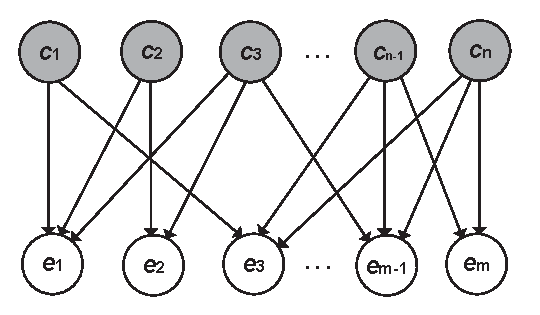
\includegraphics[width=0.9\columnwidth]{bipartition-small.eps}}
\caption{A concept-entity bipartite graph} \label{fig:bipartition}
\end{figure}

%There are some challenges in the clustering all concepts
%in the semantic network.
To cluster the concepts in the semantic network, we use the entity distributions to represent the concepts and evaluate their similarities by \eqnref{eq:semanticDist}. According to the isA relationships between concepts and entities in $\Gamma_{isA}$, we can construct a bipartite graph
between concepts and entities (Figure~\ref{fig:bipartition}) and cluster the concepts based on this graph. The basic idea is that if two
concepts share many entities, they are similar to each other. From this bipartite graph, we represent each concept $c_i$ as an L2-normalized
vector as shown in \eqnref{eq:Ic}, where each dimension corresponds to an entity in the graph.

Even though the number of concept and entity nodes may be large,
%On the surface, there are two challenges in clustering concepts
%on the bipartite graph. First, the concept nodes in this bipartite are large,
%as $\Gamma_{isA}$ consists of more than 2.7 million unique concepts.
%Therefore, the clustering algorithm must be efficient and scalable
%to handle large data sets.
%Second, the dimension $\mathcal{I}_c$ is also large, with
%over 5.5 million unique entities in $\Gamma_{isA}$.
%the data set is hence of extremely high dimensionality.
%Therefore, the clustering algorithm must tackle the
%``curse of dimensionality''.
the graph is actually very sparse.
%To overcome the above problems and find the closest cluster fast in our algorithm, we observe that the concepts in $\Gamma_{isA}$ are very sparse.
For example, a concept is connected with an average
number of 5.72 entities in $\Gamma_{isA}$. Each entity is also connected to a couple of concepts on average.
%The average degree of entities nodes is only 2.58.
Therefore, for a concept $c$, the average size of $S_c$,
the set of concepts which share at least
one entity with $c$, is small.
%is only $5.72\times (2.58-1) = 9.04$. Intuitively,
%for any cluster $C$, if $C \cap S_c = \emptyset$, \emph{C} cannot be close to $c$ since the distance of any member of \emph{C} to $c$ is 1, which is the farthest distance calculated according to \eqnref{eq:semanticDist}.
To find the closest cluster to $c$,
we only need to check the clusters which contain at
least one concept in $S_c$. Since each concept belongs to only one
cluster in our method, the average number of clusters to be checked is small.
%no more than 9.04.
%We thus use an efficient dimension array data structure\cite{Cao:2008}
%to facilitate the above checks.
Furthermore, edges in the graph with low weights (i.e., low typicality scores)
are likely to be noises and can be ignored.
%This can further simplify the graph and speed up the clustering.
%be formed due to some noisy isA relationships especially for lower co-occurrences of concepts and entities. Thus, we aim to prune these noisy concepts and entities without degrading the quality of clusters. More precisely, let $w_{ij}$ be the weight (namely the typicality score $p(e_j|c_i)$) between $c_i$ and $e_j$, let $w_i$ be the sum
%of the weights of all entities that $c_i$ contains, i.e.,
%$w_i =\sum_j w_{ij}$. We can prune an edge connecting $c_i$ and $e_j$ if the absolute
%weight the relative weight $w_{ij}/w_i < \alpha$, in our experiments,
%we set $\alpha =$ 0.001.
%After the pruning process, our clustering algorithm can finish in 15 hours when clustering 2.7 million concepts in $\Gamma_{isA}$ running on a PC of 4 GB main memory.
%


%%% Local Variables:
%%% mode: latex
%%% TeX-master: "paper"
%%% End:


\subsection{The Max-Max Similarity Function}
%We now give a general framework of measuring the semantic similarity between
%terms using the concept clustering. As shown in Algorithm \ref{alg:refined},
%our clustering-based approach also has three steps similar to the basic approach.
%% That is, we first judge the type of terms. Second, we represent the semantic contexts of each term according to its type, that is, modeling a probability distribution over contexts. Third, we compare how similar these two discrete probability distributions are by encoding them as vectors and computing the cosine between the vectors.
%The difference is that we add the clustering in Algorithm \ref{alg:conceptClustering}
%on all concept contexts of terms for their possible senses,
%and then evaluate the semantic similarity by comparing these
%concept-cluster contexts. We will give the details on the
%concept-cluster-based similarity evaluation in the following section.
%
%
%\subsubsection{Context Comparison}
In the basic approach, we compute the similarity of two terms by the
cosine similarity between their contexts (\eqnref{eq:cosine}).
In the refined approach, we use a new similarity function known as
{\em max-max similarity}.
%We formalize the concept cluster-based context comparison method as follows.
Let $C=\{C_1,C_2,...,C_k\}$ be clusters of all concepts in $\Gamma_{isA}$,
$C^{t_1}$ and $C^{t_2}$ be the sets of concepts that two terms belong to
respectively. According to the cluster information in $C$,
we divide $C^{t_1}$ and $C^{t_2}$ into small clusters
$C^{t_1}=\{C^{t_1}_{1},..., C^{t_1}_{m}\}$ and
$C^{t_2}=\{C^{t_2}_{1},..., C^{t_2}_{n}\}$ by
comparing $C^{t_1} \cap C$ and $C^{t_2} \cap C$ respectively.
We then compute the similarity between the contexts of each cluster pair
and get the semantic similarity between two terms as:
\begin{equation}
\begin{aligned}
sim(T(t_{1}), T(t_{2})) = \max_{x, y}\{cosine(C^{t_1}_{x}, C^{t_2}_{y})\}
\label{eq:clusterCosine}
\end{aligned}
\end{equation}
where $1\leq x \leq m$ and $1 \leq y \leq n$.

With all concepts clustered offline and the new similarity function
based on concept clusters, the refined algorithm is given in
Algorithm \ref{alg:refined}.
%
% \begin{table}[!h]
% \centering
% \caption{Concept clusters of a pairwise term Microsoft and Apple}% (extracted using Hearst patterns)}
% \label{tab:microsoft-apple-clusters}
% \begin{tabular}{|p{2pt}|l|c|p{2pt}|l|c|}\hline
%  & concepts &  &  & concepts & \\
% id & of Microsoft & weight & id & of Apple & weight\\\hline
% 1	&company	&0.3738	&1	&fruit	&0.2952\\
% 1	&u.s. company	&0.0349	&1	&seasonal fruit	&0.0826\\
% 1	&client	&0.0256	&1	&tree fruit	&0.0048\\
% 1	&large company	&0.0227	&1	&fresh fruit	&0.0389\\
% 1	&software giant	&0.0217	&1	&juice	&0.0067\\
% 	&international-&	&	&	&\\
% 1	&company	&0.0207	&1	&fruit juice	&0.0065\\
% 	&technology-	&	&	&	&\\
% 1	&company	&0.0145	&1	&dried fruit	&0.0051\\
% 1	&software company	&0.0141	&2	&company	&0.1239\\
% 1	&big company	&0.0125	&2	&manufacturer	&0.0100\\
% 1	&giant	&0.0123	&2	&competitor	&0.0077\\
% 1	&player	&0.0112	&2	&large company	&0.0048\\
% 1	&software vendor	&0.0095	&3	&food	&0.0612\\
% 1	&competitor	&0.0086	&3	&snack	&0.0054\\
% 1	&partner	&0.0082	&3	&healthy snack	&0.0052\\
% 1	&manufacturer	&0.0071	&4	&fruit tree	&0.0223\\
% 1	&industry giant	&0.0068	&4	&tree	&0.0083\\
% 1	&big player	&0.0063	&5	&brand	&0.0216\\
% 2	&organization	&0.0217	&6	&crop	&0.0147\\
% 3	&provider	&0.0184	&7	&flavor	&0.0121\\
% 4	&industry leader	&0.0184	&8	&product	&0.0067\\
% \hline
% \end{tabular}
% \end{table}
%
%For example, Table~\ref{tab:microsoft-apple-clusters} shows the top 20 concepts of the entity pair $<microsoft,~apple>$, according to the cluster information in $C$, we can get the clusters that each concept belongs to. In terms of Eq.~\ref{eq:clusterCosine}, we can get the maximum similarity score of this pair, namely the cosine score by comparing the context of Microsoft in the $1^{st}$ cluster with that of Apple in the $2^{nd}$ cluster. In this case, the similarity score between Microsoft and Apple is improved from 0.378 in Eq.~\ref{eq:cosine} to 0.994 in Eq.~\ref{eq:clusterCosine}.
%
%\makeatletter\def\@captype{algorithm}\makeatother
%\KZ{Is it possible to simplify this algo? The structure looks the same as
%Algo 1.} \LP{revised}

\renewcommand\algorithmicrequire{\textbf{Input:}}
\renewcommand\algorithmicensure {\textbf{Output:}}
\begin{algorithm}[th]
%\begin{center}
\caption{Refined Approach}
\label{alg:refined}
\begin{algorithmic}[1]
\REQUIRE \pair{t_1}{t_2}: a pair of terms;\\
~~~~~~$\Gamma_{isA}$: the semantic network of isA relationship;\\
~~~~~~$\Gamma_{ssyn}$: the synset data set in $\Gamma_{isA}$;\\
~~~~~~$\Gamma_{cluster}$: clusters of all concepts in $\Gamma_{isA}$;
\ENSURE a similarity score of \pair{t_1}{t_2};
\STATE Install the synset checking and type checking as Steps 1-4 in Algorithm \ref{alg:baseline};
\IF {\pair{t_1}{t_2} is a concept pair}
\STATE return $sim(\mathcal{I}_c^{t_1}, \mathcal{I}_c^{t_2})$ as Steps 6-7 in Algorithm \ref{alg:baseline};
\ENDIF
\IF {\pair{t_1}{t_2} is an entity pair}
\STATE $sim_1\leftarrow sim(\mathcal{I}_e^{t_1}, \mathcal{I}_e^{t_2})$ as Steps 10-11 in Algorithm \ref{alg:baseline};
\STATE Find clusters of contexts $C^{t_1}$ and $C^{t_2}$ from $\Gamma_{cluster}$;% and prune the cluster sets;
\STATE $sim_2\leftarrow sim(C^{t_1}, C^{t_2})$ computed in \eqnref{eq:clusterCosine};
\STATE return $max(sim_1, sim_2)$;
\ENDIF
\IF {\pair{t_1}{t_2} is a concept-entity pair}
\STATE Collect all concepts of the entity term $t_i$ from $\Gamma_{isA}$ as the context $C^{t_i} (i\in\{1, 2\})$;
\STATE Find clusters of contexts $C^{t_i}$ from $\Gamma_{cluster}$;% and prune the cluster sets;
\FOR {each cluster $C_x$ in $C^{t_i}$}
\STATE Select top $K$ concepts to represent $t_i$, namely $C{^{K}_{x}}=\{c_y|c_y \neq t_j,c_y\in C_x, 1\leq y \leq K\}$;
\FOR {each concept $c_y$ in $C{^{K}_{x}}$}
\STATE $sim_{c_y}\leftarrow$ get the semantic similarity between $c_y$ and $t_j$ by repeating this algorithm iteratively;
\ENDFOR
\STATE $sim_{C_x}\leftarrow max_{c_y\in C{^{K}_{x}}}\{sim_{c_y}\}$;
\ENDFOR
\STATE return $max\{sim_{C_x}|C_x\in C^{t_i}\}$;
\ENDIF
\end{algorithmic}
%\end{center}
\end{algorithm}


\subsection{Optimization by Cluster Pruning}
%We now discuss the advantage and disadvantage using the clustering-based approach for measuring semantic similarity between terms.
%Table~\ref{tab:examples} compares the semantic similarity scores of 9 pairs predicted in Eq.~\ref{eq:clusterCosine} and Eq.~\ref{eq:cosine}. From the experimental results, we can see that comparing the baseline approach using Eq.~\ref{eq:cosine}, our clustering-based approach using Eq.~\ref{eq:clusterCosine} ac
%tually improve the semantic similarity of pairs, such as $<Apple,~Microsoft>$, $<Orange,~Red>$ and $<Microsoft, GE>$ those with ambiguous terms whose data d
%istributions of senses hidden in contexts are skewed. However, it also improves the similarity score of dissimilar pairs like $<lunch,~music>$. This is cause by the following reasons.
The cluster-based refined approach improves the quality of similarity remarkably from
the basic algorithm. But there are two problems. First, the max-max similarity function tends to boost the probability of picking
a less dominant sense of a term because it is easier for 
small clusters to look similar
by the cosine similarity and hence dominate the max-max similarity score. However, many small clusters in $C$ are usually noises. This leads to incorrect
similarity results.
%
%First, there are some noisy concepts in the tail of the concept context given a term, which lead to many small sized clusters formed when using the offline
%clustering method.
%For example, as shown in Table~\ref{tab:microsoft-apple-clusters}, there are small clusters like crop and flavor in the top 20 concepts of Apple, which does
% not accurately represent a sense of Apple.
Second, with the current concept clustering algorithm, some terms can have both
a general sense and a more specific sense. For example, the term ``lunch'' has a specific
sense called ``dish'' and a more general (and also vague) sense called ``activity''.
We know ``activity'' is  more general because it is a superconcept of ``disk''
in $\Gamma_{isA}$. Such general senses poses problems because they make almost
unrelated terms similar. For example, the term ``music'' also has the ``activity'' sense
and thus is deemed similar to ``lunch''.
%
%some term we can get some general (vague) senses except of specific senses when clustering the concept context, because we clustering all concepts flatly. For
% example, considering the senses of Music and Lunch as shown in Table~\ref{tab:sensesOfSamples}, we call the Activity sense as a vague sense and the dish and multimedia senses as specific ones. This is because the former is a super concept of the latter according to the isA relationships in $\Gamma_{isA}$, whose importance as the sense of the term is less than the latter.
%

To overcome these problems, we adopt an optimization technique called
{\em cluster pruning} after concept clustering.
First, to reduce the negative impact from noisy clusters,
we prune away those clusters with only one member or with very small combined weight.
% the weight is lower than the threshold $\tau$ (e.g., 0.01).
%We use the normalized sum typicality of scores for the term \emph{e}
%and its concept $c_i$ in a cluster $C_x$ as the weight of the current cluster.
The weights of clusters are computed below. Let the concept clusters of the term \emph{t} be $C^t = \{C^t_1,...,C^t_m\}$,
the weight of each cluster $C_x^{t}$ is $w_x/\sum_{x}w_x$, where
$w_x = \sum_{c_i\in C_x^{t}}p(c_i|t)$ and $1 \leq x \leq m$.
%In this processing, we can get more accurate senses for each terms. For example, Table~\ref{tab:sensesOfSamples} summarizes main senses of ambiguous terms in Table~\ref{tab:examples} according to the cluster centers and their weights.
Second, to avoid the impact from the vague senses, we prune the clusters
whose senses are superconcepts of other senses according to the isA relationships
in $\Gamma_{isA}$. For example, Fig.~\ref{fig:clusters-given-a-pair}
shows a hierarchical isA relationships of senses after clustering concept
contexts of two terms ``lunch'' and ``music''. Because the senses ``Activity'',
``Cost'', ``Interest'' and ``Art'' are the superconcepts of the senses ``Dish'' and
``Multimedia'', we only keep specific senses like ``Dish'' and ``Multimedia'' and
remove the rest.
%then we compare their contexts in the clusters in Eq.~\ref{eq:clusterCosine}.
%Finally, we can get the similarity between Lunch and Music,
%which is reduced to \textbf{0.012}.

%\begin{table}[!t]
%\centering
%\caption{Main senses of sampling terms}
%\label{tab:sensesOfSamples}
%\begin{tabular}{|c|c|c|c|} \hline
%entity &id &	senses	&weight\\\hline
%	&1	&Fruit & 0.792\\
%Apple	&2	&Company &0.138\\
%	&3	&Fruit Tree & 0.080\\\hline
%	&1	&Fruit & 0.457\\
%Orange	&2	&Color &0.447\\
%	&3	&Company&0.014\\\hline
%GE	&1	&Company & 0.606\\
%	& 2	&Material&0.394\\\hline
%	&1	&Interest &0.518\\
%Music	&2	&Multimedia&0.201\\
%	&3	&Activity & 0.196\\
%	&4	&Art&0.085\\\hline
%	&1	&Dish &0.501\\
%Music	&2	&Activity&0.251\\
%	&3	&Cost&0.248\\\hline
%Pear	&1	&Fruit & 0.824\\
%	&2	&Fruit Tree & 0.097\\\hline
%Microsoft	&1	&Company &0.895\\\hline
%\end{tabular}
%\end{table}

\begin{figure}[th]
 \centerline{
 \includegraphics[width=0.9\columnwidth]{clusters-given-a-pair.eps}}
\caption{Illustration to vague and specific senses of terms lunch and music} \label{fig:clusters-given-a-pair}
\end{figure}





%%% Local Variables:
%%% mode: latex
%%% TeX-master: "paper"
%%% End:

\section{Experiments}
\label{sec:eval}

%In this section, we evaluate the effectiveness and efficiency of
%our approach in computing the semantic similarity between terms.
In this section, we first outline the experimental setup and give the parameter analysis for several important parameters involved in our approaches, 
and then compare the effectiveness of the online and the offline
variant of our approach, and also compare our approaches
(basic, refined and refined with pruning) with 12 competing
methods on three benchmark data sets.
Finally, we evaluate the efficiency of our approaches.
% in the context of other peers.

\subsection{Experiment Setup}
We use three data sets in the following experiments, including two well-known benchmark data sets for word similarity and one labeled data set
for evaluating MWEs which is created by us. Table~\ref{tab:dataSets} shows the descriptions and some examples in each of the three data sets.
M\&C data set is a subset of Rubenstein-Goodenough's \cite{Rubenstein:1965}
and consists of 28 word pairs.
Because of the omission of two word
pairs in earlier versions of WordNet, most researchers used only
28 word pairs for evaluations in the past. We follow this tradition in this paper.
WordSim203 is a subset from WordSim353\cite{wordSim:353}, and has been
used as a similarity testing data set\cite{Agirre:2009} by Agirre et. al.
It contains 203 pairs which are considered more similar than related.
These similar pairs include those
classified as synonyms, antonyms, identical, or hyponym-hypernym, and unrelated pairs indicate those classified as none-of-the-above that have average similarity less than or equal to 0.5 (on a scale of 0 to 1).
Because there are no benchmark data for the semantic similarity between
MWEs, we labeled 300 pairs (known as WP) with both words and MWEs. Our labeled data consist of three categories: 100 concept-entity pairs, 100
concept-concept pairs and 100 entity-entity pairs. These 300 pairs contain 84 word pairs and 216 MWE pairs, in which 71 MWE pairs are in WordNet
the remaining are not. You can find all 300 labeled pairs at \url{http://adapt.seiee.sjtu.edu.cn/similarity/SimCompleteResults.pdf}.
%and the composition of word/MWE pairs is listed
%in Table~\ref{tab:pairDistribution}.
Five native speakers of English labeled these pairs according to the label classes, and the labels are then translated into numerical similarity
scores in Table~\ref{tab:manualLabels}. These scores are averaged to produce
the final rating for each pair.

All experiments are performed on
an Intel Core 2 Duo 2.66GHz PC with 4G physical memory,
running Windows 7 Enterprise. All timing results are averaged over 10 runs.
All competing methods involved in this section are summarized
in Table~\ref{tab:allmethods}. We implemented S\'{a}n method while adopting the existing implementation \cite{wordNetSim} of other methods.
%open source code at authors' homepage or they are encapsulated in an open source tool for WordNet-based similarity\cite{wordNetSim}.
To evaluate the effectiveness of each method,
we compute the Pearson Correlation Coefficient (PCC in short)
to measure the agreement between the machine rating
(computed by the semantic similarity measurement approaches) and
the human ratings over the data sets
as follows, where
$X$ is the machine ratings while $Y$ is the human ratings:
\begin{eqnarray*}\label{eq:PCC}
 \rho = \frac{\sum_{i=1}^n(X_i-\bar{X})(Y_i-\bar{Y})}{\sqrt{\sum_{i=1}^n(X_i-\bar{X})^2}\sqrt{\sum_{i=1}^n(Y_i-\bar{Y})^2}}
\end{eqnarray*}

In the following subsections, we first give the parameter analysis relevant to the parameters in k-Medoids and our proposed algorithms, then give the experiments on the selection of similarity function $F(\cdot)$ as shown in Eq.~\ref{eq:F}. Finally, we report the experimental results of our algorithms on the effectiveness and efficiency based on the previous experimental conclusions.

\begin{table}[th]
\centering
\caption{Data Sets Used in Experiments}
\label{tab:dataSets}
\small
\begin{tabular}{|c|c|c|}\hline
 M\&C   &WordSim203 similarity &Our labeled data\\
 data set\cite{Miller:1998} &\cite{Agirre:2009}(WS in short) &(WP in short)\\\hline\hline
 \multicolumn{3}{|l|}{~~~~~~~~~~~~~~~~~~~~~~~~~~~~~~~~~~\textbf{Type}}\\\hline
 Words & Words & Words \& MWEs \\\hline
 \multicolumn{3}{|l|}{~~~~~~~~~~~~~~~~~~~~~~~~~~~~~~~~~\textbf{\#Pairs}}\\\hline
  28 & 203 & 300 \\\hline
  \multicolumn{3}{|l|}{~~~~~~~~~~~~~~~~~~~~~~~~~~~~~~~\textbf{Examples}}\\\hline
 \pair{lobster}{food} &\pair{lobster}{wine}&\pair{animal}{poodle}\\\hline
\pair{chord}{smile} &\pair{professor}{doctor}&\pair{microsoft}{apple}\\\hline
&&$\langle$\emph{shell},~\emph{exxon}\\
\pair{bird}{cock} &\pair{tiger}{jaguar}&\emph{mobil~corp.}$\rangle$\\\hline
$\langle$\emph{crane},  &   &$\langle$\emph{caged~animal},\\
\emph{implement}$\rangle$   &$\langle$\emph{precedent},\emph{information}$\rangle$   &\emph{game~animal}$\rangle$\\\hline
\end{tabular}
\end{table}

%\begin{table}[th]
%\centering
%\caption{Experimental Data}
%\label{tab:dataSets}
%\scriptsize{
%\begin{tabular}{|c|c|c|c|}\hline
% &     &WordSim353  &\\
%  & M\&C   &similarity\cite{wordSim:353} &Our labeled data\\
% & database\cite{Miller:1998}  &(WS for short) &(WP for short)\\\hline\hline
%Type & Words & Words & Words \& MWEs \\\hline
%\#Pairs & 28 & 203 & 300 \\\hline
% &\pair{lobster}{food} &\pair{cup}{artifact}&\pair{animal}{poodle}\\\cline{2-4}
%&\pair{chord}{smile}   &\pair{doctor}{nurse}&\pair{microsoft}{apple}\\\cline{2-4}
%&&&$<$\emph{shell},~\emph{exxon}\\
%Examples&\pair{coast}{forest} &\pair{football}{tennis}&\emph{mobil~corp.}$>$\\\cline{2-4}
%&$<$\emph{crane},  &$<$\emph{deployment},  &$<$\emph{caged~animal},\\
%&\emph{implement}$>$   &\emph{departure}$>$    &\emph{game~animal}$>$\\\hline
%\end{tabular}
%}
%\end{table}

%\begin{table}[!t]
%\centering
%\caption{Experimental Data}
%\label{tab:dataSets}
%\small{
%\begin{tabular}{|c|c|c|c|}\hline
%Data source & type &\#pairs &Description\\\hline
%&  & & Judged by 51 human subjects\\
%database & word &28 & in a scale of [0.0, 4.0]\\\hline
%&  & & An average of 13-16 human\\
%(WS for short)\cite{wordSim:353} & word &203 &judgements in a scale of [0.0, 10.0]\\\hline
%& word and multi- & &An average of 5 human\\
%(WP for short)& word expression & 300& judgements in a scale of [0.0, 1.0]\\\hline
%\end{tabular}
%}
%\end{table}
%\begin{table}[!t]
%\centering
%\caption{Some Examples from Three databases}
%\label{tab:samplesOfDatasets}
%\small{
%\begin{tabular}{|c|c|c|}\hline
%M\&C database & WordSim353 similarity  &WP database\\\hline
%\pair{lobster}{food}   &\pair{cup}{artifact}   &\pair{microsoft}{apple}\\
%\pair{coast}{forest}   &\pair{deployment}{departure}   &\pair{marine animal}{cold-blooded animal}\\
%\pair{crane}{implement}    &\pair{doctor}{nurse}   &\pair{animal}{poodle}\\
%\pair{chord}{smile}    &\pair{football}{tennis}    &\pair{shell}{exxon mobil corp.}\\\hline
%\end{tabular}
%}
%\end{table}

%\begin{table}[th]
%\centering
%\caption{Distributions of Pairs in WP}
%\label{tab:pairDistribution}
%\small{
%\begin{tabular}{|c|c|c|c|}\hline
%&Word & MWE & Total\\\hline\hline
%\#Pairs &84 & 216 & 300\\
%\#Identified by WordNet & 75 & 71&146\\\hline
%\end{tabular}
%}
%\end{table}

\begin{table}[th]
\centering
\caption{Label Classes and Similarity Scores}
\label{tab:manualLabels}
\small{
\begin{tabular}{|c|c|}\hline
Label Classes   & Similarity Score\\\hline\hline
Very similar    &1\\
Fairly similar  &0.75\\
Don't know  &0.5\\
Fairly different    &0.25\\
Very different  &0\\\hline
\end{tabular}
}
\end{table}

\subsection{Parameter Analysis}
In this subsection, we will observe the experiments on several main parameters relevant to k-Medoids and our proposed algorithms, including the thresholds $\alpha$, \emph{topK} and $max_{Depth}$.
In the above analysis, we get that the threshold $\alpha$ is related to the number of clusters and the prediction result of PCC on the concept-entity pairs, values of \emph{topK} and $max_{Depth}$ are related to the computation time and the prediction result of PCC on the concept-entity pairs. Because the experimental conclusions about these three parameters are irrelevant to the concise similarity function $F(\cdot)$, the following experiments are conducted using the similarity function $F(\cdot)=cosine$.

Figure \ref{fig:a} reports the curves of the cluster count on three data sets varying with the values of $\alpha$ from 0.05 to 0.95 with a 0.05 step. Experimental results show that as the value of $\alpha$ increases, the count of clusters are linearly decreasing. The reason is clear corresponding to the constraint in Eq.~\ref{eq:initMedoid}. Meanwhile, we conduct the experiments of PCC values on three data sets varying with the cluster counts as shown in this figure. We find that the largest variance of PCC values on each data set is more than 0.15 while the count of clusters varies from 29,483 to 4,628 with the increasing of the PCC values. However, when the value of $\alpha$ varies from 0.6 to 0.8, the cluster count correspondingly varies from 15,000 to 10,000, in this case, the fluctuation of the PCC value is more gentle. That is, the variance of PCC value on the M\&C data set is no more than 0.035 while the variances of PCC values on the WS and WP data sets are no more than 0.005. Thus, we get a conclusion that the optimal value of $\alpha$ ranges from 0.6 to 0.8. In our experiments, we select the value of $\alpha = $0.7 as an optimal value in the clustering algorithm of k-Medoids.

Figure \ref{fig:topK} reports the curves of the PCC value and the mean computation time on the concept-entity pairs varying with the values of $topK$ from 1 to 20 with a step of 1. Experimental results show that as the value of $topK$ increases from 1 to 20, the mean computation time on each concept-entity pair is linearly increasing, while the PCC values first increase to a peak value, then decrease to a stable value. To trade-off these two evaluation measures, namely maintaining a higher value of PCC and a lower value of the mean computation time, we select the optimal value of $topK $= 3 in our experiments.

Figure \ref{fig:maxDepth} reports the curves of the PCC value and the mean computation time on the concept-entity pairs varying with the values of $max_{Depth}$ from 1 to 20 with a step of 1. In the observation of experimental results, we can see that as the value of $max_{Depth}$ increases from 1 to 20, the computation time on each concept-entity pair is averagely increasing up to a stable value, while the PCC values first increase to a peak value, then decrease to a stable value. This is because all concept-entity pairs used here have no deep parent-child relationships, in our experiments, the largest depth of parent-child relationships is no more than 7 level. Hence, when the value of $max_{Depth}$ increases up to a larger value (e.g. 7), experimental results relevant to the PCC values and the mean computation time maintain stability. To trade-off these two evaluation measures, namely maintaining a higher value of PCC and a lower value of the mean computation time, we select the optimal value of $max_{Depth} $= 3 in our experiments.

\begin{figure}[!t]
 \centerline{
 \includegraphics[width=0.9\columnwidth]{relationship-between-a-and-others.eps}}
 \caption{Relationship between $\alpha$ and cluster count and PCC values}
 \label{fig:a}
\end{figure}

\begin{figure}[!t]
 \centerline{
 \includegraphics[width=0.8\columnwidth]{topK-relationships.eps}}
 \caption{Relationship between $topK$ and PCC values and computation time}
 \label{fig:topK}
\end{figure}

\begin{figure}[!t]
 \centerline{
 \includegraphics[width=0.8\columnwidth]{maxDepth-relationships.eps}}
 \caption{Relationship between $max_{Depth}$ and PCC values and computation time}
 \label{fig:maxDepth}
\end{figure}

%the best trade-off value between the PCC value and the mean computation time in our algorithms. ?
\subsection{Selection on the Similarity Function $F(\cdot)$}
In this subsection, we will observe the experiments of PCC values conducted on three data sets in different similarity functions as $F(\cdot)$, including cosine, Jaccard, JaccardExtended, JS\_Sim and KL\_Sim, where $JS\_Sim$ indicates Jensen-Shannon divergence based similarity function and $KL\_Sim$ indicates smoothed Kullback\-Leibler divergence based similarity function.

We first give the definitions on the specified similarity functions mentioned above. That is, given two vectors $X = \{x_1, ...,x_m\}$ and $Y=\{y_1,...,y_n\}$, the relevant similarity functions are defined below, where the outcome of each similarity function is neatly bounded in [0,1].

$$cosine(X,Y) = \frac{||X\cdot Y||}{||X||_2^2\cdot ||Y||_2^2}$$
$$Jaccard(X,Y) = \frac{|X\cap Y|}{|X|+|Y|-|X\cap Y|}$$
$$JaccardExtended(X,Y) = \frac{\Sigma_{i=1}^{|X\cap Y|}(x_i+y_i)}{\Sigma_{i=1}^mx_i+\Sigma_{j=1}^ny_j}$$
$$KL\_Sim(X,Y) = 1-Normalized(KL(X,Y))$$
$$~with~KL(\cdot)=\Sigma_{i=1}^{|X\cap Y|}(x_i\cdot log_2(x_i/y_i))$$
$$JS\_Sim(X,Y) = 1-\frac{KL(X,M) + KL(Y, M)}{2} ~(M = \frac{X+Y}{2})$$

Figure \ref{fig:F} reports the performances of our RCP algorithm varying with five different similarity functions. Experimental results show that on the data sets of M\&C and WS, the PCC value of our RCP algorithm performs worst in the similarity function based on KL divergence, but there is little variance compared to those in similarity functions based on cosine, jaccard, jaccardExtended and JS divergence. The largest variance is no more than 0.01. However, on the WS data set, RCP using the similarity functions of cosine and jaccardExtended outperforms that using the similarity fucntions of jaccard, JS divergence and KL divergence, more precisely, the PCC value is improved up to 0.06. These data reveal that our algorithm using the similarity functions of cosine and jaccardExtended is more superior to others. In the following experiments, we select the cosine similarity function as the function of $F(\cdot)$ used in Eq.~\ref{eq:F}.

\begin{figure}[!t]
 \centerline{
 \includegraphics[width=0.8\columnwidth]{similarity-function-selection.eps}}
 \caption{Performance comparison varying with five similarity functions}
 \label{fig:F}
\end{figure}

\begin{table}[th]
\centering
\caption{Competing Methods (IC = Information Content, LCA = Least Common Ancestor)}
\label{tab:allmethods}
\small
\begin{tabular}{|l|l|}\hline
{\bf Approach} & {\bf Description} \\\hline\hline
Hungarian (Hun) \cite{hungarian:string}     &string-based\\\hline
Tray (Tra)\cite{tray:2005} &string-based+WordNet \\ \hline
Rada (Rad) \cite{Rada:1989} &path-based (WordNet) \\\hline
Hirst (Hir) \cite{Hirst:1998}   &lexical chain-based (WordNet) \\\hline
Do \cite{Do:DRSTV09}    &lexical chain-based (WordNet) \\\hline
Resnik (Res)\cite{Resnik:1995}  & IC of LCA $+$WordNet \\\hline
Jcn \cite{Jiang:1997}   & IC of LCA + the term + WordNet \\\hline
Lin \cite{Lin:1998} & IC of LCA + the term + WordNet\\\hline
S\'{a}nchez (S\'{a}n)\cite{Snchez:2011} & IC of leaves and parents + WordNet \\\hline
Banerjee (Ban)\cite{Banerjee:2002}  & glosses-based (WordNet) \\\hline
Agirre (Agi)\cite{Agirre:2010}  & personalized PageRank (WordNet)\\\hline
Bollegala (Bol)\cite{Bollegala:2011} &search-snippet-based  \\\hline
Basic & Our basic approach\\\hline
RC & Our refined approach \\\hline
RCP & Our refined approach with pruning \\\hline
\end{tabular}
\end{table}

%\begin{table*}[th]
%\centering
%\caption{Pearson Correlation Coefficient on Three Data Sets
%with Word or MWE pairs}
%\label{tab:benchmarkData}
%\small{
%\begin{tabular}{|c|c|c|c|c|c|c|c|}\hline
%%  &   \multicolumn{3}{c|}{} &\multicolumn{2}{c|}{Pairs with multi-}\\
%&  \multicolumn{4}{c|}{Word Pairs} &\multicolumn{3}{c|}{MWE Pairs}\\\hline
%   &   & &75 pairs & total 278 pairs &71 pairs & 145 pairs &total 216 pairs \\ %&146 pairs\\
%Method &M\&C &WS & in WordNet & &in WordNet &not in WordNet &  \\ \hline\hline % & in WP\\\hline\hline
%Hun    &-0.196 &0.064 &0.039&0.049 &0.371 &0.429&0.355\\ \hline % &0.093\\\hline
%Tra    &0.755  &0.594 &0.520&0.579 &0.389 &0.325&0.344\\ \hline %&0.459\\\hline
%Rad&0.739  &0.595&0.520&0.569&0.592    &-&-\\ \hline %&0.557\\\hline
%Hir    &0.643  &0.574&0.533&0.552&0.459    &-&-\\ \hline %&0.504\\\hline
%Do &0.676  &0.482&0.355&0.440&0.359    &-&-\\ \hline %&0.344\\\hline
%Res&0.762  &0.672&0.573&0.643&0.744    &-&-\\ \hline %&0.677\\\hline
%Jcn&0.848  &0.371&0.641&0.285&0.382    &-&-\\ \hline %&0.432\\\hline
%Lin&0.822  &0.674&0.605&0.658&0.717    &-&-\\ \hline %&0.678\\\hline
%San&0.865  &0.690  &0.675  &0.681&0.740    &-&-\\ \hline %&0.701\\\hline
%Ban&0.781  &0.651&0.470&0.594&0.377     &-&-\\ \hline %&0.428\\\hline
%Agi&0.795  &0.579&0.570&0.359&0.380     &-&-\\ \hline %&0.465\\\hline
%Bol&0.834  &0.564& 0.466&0.523&0.592 &0.511&0.498\\ \hline %& 0.478\\\hline
%Basic&0.777    &0.576 &0.321&0.446&0.313    &0.449&0.440\\ \hline %&0.356\\\hline
%RC &0.885  &0.690 &0.452&0.484&0.651    &0.635&0.595\\ \hline %&0.520\\\hline
%RCP&\textbf{0.921}&\textbf{0.725} &\textbf{0.772}&\textbf{0.767}&\textbf{0.822} &\textbf{0.665}&\textbf{0.670}\\ \hline %&\textbf{0.760}\\\hline
%\end{tabular}
%}
%\end{table*}
%
%\begin{table}[th]
%\centering
%\caption{Pearson Correlation Coefficient on Three Data Sets}
%\label{tab:benchmarkData}
%\small{
%\begin{tabular}{|c|c|c|c|c|}\hline
%%  &   \multicolumn{3}{c|}{} &\multicolumn{2}{c|}{Pairs with multi-}\\
%   &   & &terms from WP &terms from WP not \\ %&146 pairs\\
%Method &M\&C &WS & in WordNet &in WordNet   \\ \hline\hline % & in WP\\\hline\hline
%Hun    &-0.196 &0.064 &0.093 &0.429\\ \hline % &0.093\\\hline
%Tra    &0.755  &0.594 &0.459 &0.325\\ \hline %&0.459\\\hline
%Rad&0.739  &0.595&0.557    &-\\ \hline %&0.557\\\hline
%Hir    &0.643  &0.574&0.504   &-\\ \hline %&0.504\\\hline
%Do &0.676  &0.482&0.344    &-\\ \hline %&0.344\\\hline
%Res&0.762  &0.672&0.677   &-\\ \hline %&0.677\\\hline
%Jcn&0.848  &0.371&0.432    &-\\ \hline %&0.432\\\hline
%Lin&0.822  &0.674&0.678   &-\\ \hline %&0.678\\\hline
%S\'{a}n&0.865  &0.690  &0.715      &-\\ \hline %&0.701\\\hline
%Ban&0.781  &0.651&0.428    &-\\ \hline %&0.428\\\hline
%Agi&0.795  &0.579&0.465    &-\\ \hline %&0.465\\\hline
%Bol&0.834  &0.564& 0.478 &0.511\\ \hline %& 0.478\\\hline
%Basic&0.777    &0.576 &0.356   &0.449\\ \hline %&0.356\\\hline
%RC &0.885  &0.690 &0.520   &0.635\\ \hline %&0.520\\\hline
%RCP&\textbf{0.921}&\textbf{0.725} &\textbf{0.760}&\textbf{0.665}\\ \hline %&\textbf{0.760}\\\hline
%\end{tabular}
%}
%\end{table}

%\begin{table*}[th]
%\centering
%\caption{Pearson Correlation Coefficient on Three Data Sets
%with Word or MWE pairs}
%\label{tab:benchmarkData}
%\small{
%\begin{tabular}{|c|c|c|c|c|c|c|c|}\hline
%  &   \multicolumn{3}{c|}{} &\multicolumn{2}{c|}{Pairs with multi-}\\
%&  \multicolumn{4}{c|}{Word Pairs} &\multicolumn{3}{c|}{MWE Pairs}\\\hline
%   &   & &75 pairs & total 278 pairs &71 pairs & 145 pairs &total 216 pairs \\ %&146 pairs\\
%Method &M\&C &WS & in WordNet & &in WordNet &not in WordNet &  \\ \hline\hline % & in WP\\\hline\hline
%Hun    &-0.196 &0.064 &0.039&0.049 &0.371 &0.429&0.355\\ \hline % &0.093\\\hline
%Tra    &0.755  &0.594 &0.520&0.579 &0.389 &0.325&0.344\\ \hline %&0.459\\\hline
%Rad&0.739  &0.595&0.520&0.569&0.592    &-&-\\ \hline %&0.557\\\hline
%Hir    &0.643  &0.574&0.533&0.552&0.459    &-&-\\ \hline %&0.504\\\hline
%Do &0.676  &0.482&0.355&0.440&0.359    &-&-\\ \hline %&0.344\\\hline
%Res&0.762  &0.672&0.573&0.643&0.744    &-&-\\ \hline %&0.677\\\hline
%Jcn&0.848  &0.371&0.641&0.285&0.382    &-&-\\ \hline %&0.432\\\hline
%Lin&0.822  &0.674&0.605&0.658&0.717    &-&-\\ \hline %&0.678\\\hline
%San&0.865  &0.690  &0.675  &0.681&0.740    &-&-\\ \hline %&0.701\\\hline
%Ban&0.781  &0.651&0.470&0.594&0.377     &-&-\\ \hline %&0.428\\\hline
%Agi&0.795  &0.579&0.570&0.359&0.380     &-&-\\ \hline %&0.465\\\hline
%Bol&0.834  &0.564& 0.466&0.523&0.592 &0.511&0.498\\ \hline %& 0.478\\\hline
%Basic&0.777    &0.576 &0.321&0.446&0.313    &0.449&0.440\\ \hline %&0.356\\\hline
%RC &0.885  &0.690 &0.452&0.484&0.651    &0.635&0.595\\ \hline %&0.520\\\hline
%RCP&\textbf{0.921}&\textbf{0.725} &\textbf{0.772}&\textbf{0.767}&\textbf{0.822} &\textbf{0.665}&\textbf{0.670}\\ \hline %&\textbf{0.760}\\\hline
%\end{tabular}
%}
%\end{table*}

%\begin{table*}[th]
%\centering
%\caption{Pearson Correlation Coefficient on Three Data Sets
%with Word or MWE Pairs}
%\label{tab:benchmarkData1}
%\small{
%\begin{tabular}{|c|c|c|c|c||c|c|c|}\hline
%%	&	\multicolumn{3}{c|}{} &\multicolumn{2}{c|}{Pairs with multi-}\\
%&	\multicolumn{4}{c||}{Word Pairs} &\multicolumn{3}{c|}{MWE Pairs}\\\hline
%	&	& & Words & & MWE Pairs & MWE Pairs & \\ %&146 pairs\\
%Method	&M\&C &WS & from WP & All Word Pairs &in WordNet &Not in WordNet & All MWE Pairs \\ \hline\hline % & in WP\\\hline\hline
%Hun	&-0.196	&0.064 &0.015&0.038 &0.371 &0.429&0.355\\ \hline % &0.093\\\hline
%Tra	&0.755	&0.594 &0.379&0.480 &0.389 &0.325&0.344\\ \hline %&0.459\\\hline
%Rad&0.739	&0.595&0.395&0.510&0.592	&-&-\\ \hline %&0.557\\\hline
%Hir	&0.643	&0.574&0.451&0.511&0.459	&-&-\\ \hline %&0.504\\\hline
%Do	&0.676	&0.482&0.322&0.419&0.359	&-&-\\ \hline %&0.344\\\hline
%Res&0.762	&0.672&0.424&0.569&0.744	&-&-\\ \hline %&0.677\\\hline
%Jcn&0.848	&0.371&0.382&0.275&0.382	&-&-\\ \hline %&0.432\\\hline
%Lin&0.822	&0.674&0.446&0.579&0.717	&-&-\\ \hline %&0.678\\\hline
%S\'{a}n&0.865	&0.690	&0.643&0.655&0.740	&-&-\\ \hline %&0.701\\\hline
%Ban&0.781	&0.651&0.426&0.560&0.377	 &-&-\\ \hline %&0.428\\\hline
%Agi&0.795	&0.579&0.258&0.343&0.380	 &-&-\\ \hline %&0.465\\\hline
%Bol&0.834	&0.564& 0.476&0.523&0.592 &0.511&0.498\\ \hline %& 0.478\\\hline
%Basic&0.777	&0.576 &0.387&0.429&0.313	 &0.449&0.440\\ \hline %&0.356\\\hline
%RC	&0.885	&0.690 &0.457&0.494&0.651	 &0.635&0.595\\ \hline %&0.520\\\hline
%RCP&\textbf{0.921}&\textbf{0.725} &\textbf{0.811}&\textbf{0.770}&\textbf{0.822} &\textbf{0.665}&\textbf{0.670}\\ \hline %&\textbf{0.760}\\\hline
%\end{tabular}
%}
%\end{table*}

%\begin{table}[th]
%\centering \caption{Pearson Correlation Coefficient on Three Data Sets with Word or MWE Pairs (WN: WordNet)} \label{tab:benchmarkData}
%\scriptsize{
%\begin{tabular}{|p{23pt}|p{18pt}|p{15pt}|p{19pt}|p{16pt}||p{21pt}|p{23pt}|p{17pt}|}\hline
%%   &   \multicolumn{3}{c|}{} &\multicolumn{2}{c|}{Pairs with multi-}\\
%&   \multicolumn{4}{c||}{Word Pairs} &\multicolumn{3}{c|}{MWE Pairs}\\\hline
%    &   & & Words &~All& MWEs &  MWEs &~All\\ %&146 pairs\\
%Method  &M\&C &WS &~from  &  Word  &~~~in  &Not in  &  MWE \\
%  && &~WP &  Pairs &~~WN & ~~WN & Pairs \\
%\hline\hline % & in WP\\\hline\hline
%Hun &-0.20 &0.06 &0.02&0.04 &0.37 &0.43&0.36\\ \hline % &0.093\\\hline
%Tra &0.76  &0.59 &0.38&0.48 &0.39 &0.33&0.34\\ \hline %&0.459\\\hline
%Rad&0.74   &0.60&0.40&0.51&0.59    &-&-\\ \hline %&0.557\\\hline
%Hir &0.64  &0.57&0.45&0.51&0.46    &-&-\\ \hline %&0.504\\\hline
%Do  &0.68  &0.48&0.32&0.42&0.36    &-&-\\ \hline %&0.344\\\hline
%Res&0.76   &0.67&0.42&0.57&0.74    &-&-\\ \hline %&0.677\\\hline
%Jcn&0.85   &0.37&0.38&0.28&0.38    &-&-\\ \hline %&0.432\\\hline
%Lin&0.82   &0.67&0.45&0.58&0.72    &-&-\\ \hline %&0.678\\\hline
%S\'{a}n&0.87   &0.69  &0.64&0.66&0.74  &-&-\\ \hline %&0.701\\\hline
%Ban&0.78   &0.65&0.43&0.56&0.38     &-&-\\ \hline %&0.428\\\hline
%Agi&0.80   &0.58&0.26&0.34&0.38     &-&-\\ \hline %&0.465\\\hline
%Bol&0.83   &0.56& 0.48&0.52&0.59 &0.51&0.50\\ \hline %& 0.478\\\hline
%Basic&0.78 &0.58 &0.39&0.43&0.31    &0.45&0.44\\ \hline %&0.356\\\hline
%RC  &0.89  &0.69 &0.46&0.49&0.65    &0.64&0.60\\ \hline %&0.520\\\hline
%RCP&\textbf{0.92}&\textbf{0.73} &\textbf{0.81}&\textbf{0.77}&\textbf{0.82} &\textbf{0.67}&\textbf{0.67}\\ \hline %&\textbf{0.760}\\\hline
%\end{tabular}
%}
%\end{table}

%\begin{table*}[!t]
%\centering
%\caption{Pearson correlation coefficient on 146 labeled data identified by WordNet}
%\label{tab:146pairs}
%\begin{tabular}{|l|l|c|c|c|}\hline
%~~~~~~~~~Approach  &~~~~~~~~~~~~~~~Source  &on 75 pairs    &on 71 pairs    &on 146 pairs\\\hline
%Hungarian method   &string-based   &0.0391 &0.3712&    0.0931\\\hline
%Tray's (2005)  &string-based+WordNet   &0.5201 &0.3887 &0.4594\\\hline
%Rada's (1989)  &path-length-based (WordNet)    &0.5195 &0.5915 &0.5568\\\hline
%Hirst's (1998) &lexical chain-based  (WordNet) &0.5334 &0.4586 &0.5036\\\hline
%Do's (2009)    &lexical chain-based (WordNet)  &0.3550 &0.3586 &0.3438\\\hline
%resnik's (1995)    &information content+WordNet    &0.5727 &0.7438 &0.6773\\\hline
%jcn's (1997)   &information content+WordNet    &0.6408 &0.3819 &0.4319\\\hline
%lin's (1998)   &information content+WordNet    &0.6048 &0.7169 &0.6777\\\hline
%Banerjee's (2002)  &glosses-based (WordNet)    &0.4698 &0.3768 &0.4279\\\hline
%Eneko's (2010) &personalized PageRank (WordNet)    &0.5696 &0.3802 &0.4650\\\hline
%our basic approach &semantic network-based &0.3212 &0.3125 &0.3557\\\hline
%clustering-based &semantic network+clustering  &0.4521 &0.6506 &0.5195\\\hline
%our clustering approach    &semantic network+clustering+clusterPrunning    &\textbf{0.7716}     &\textbf{0.8215}   &\textbf{0.7601}\\\hline
%\end{tabular}
%\end{table*}
\begin{table}[th]
\centering
\caption{Pearson Correlation Coefficient on Word Pairs}
\label{tab:benchmarkData1}
\small{
\begin{tabular}{|c|c|c|c|c|}\hline
%	&	\multicolumn{3}{c|}{} &\multicolumn{2}{c|}{Pairs with multi-}\\
&	\multicolumn{4}{c|}{Word Pairs} \\\hline
	&	& & Words &  \\ %&146 pairs\\
Method	&M\&C &WS & from WP & All Word Pairs  \\ \hline\hline % & in WP\\\hline\hline
Hun	&-0.196	&0.064 &0.015&0.038 \\ \hline % &0.093\\\hline
Tra	&0.755	&0.594 &0.379&0.480 \\ \hline %&0.459\\\hline
Rad&0.739	&0.595&0.395&0.510\\ \hline %&0.557\\\hline
Hir	&0.643	&0.574&0.451&0.511\\ \hline %&0.504\\\hline
Do	&0.676	&0.482&0.322&0.419\\ \hline %&0.344\\\hline
Res&0.762	&0.672&0.424&0.569\\ \hline %&0.677\\\hline
Jcn&0.848	&0.371&0.382&0.275\\ \hline %&0.432\\\hline
Lin&0.822	&0.674&0.446&0.579\\ \hline %&0.678\\\hline
S\'{a}n&0.865	&0.690	&0.643&0.655\\ \hline %&0.701\\\hline
Ban&0.781	&0.651&0.426&0.560\\ \hline %&0.428\\\hline
Agi&0.795	&0.579&0.258&0.343\\ \hline %&0.465\\\hline
Bol&0.834	&0.564& 0.476&0.523\\ \hline %& 0.478\\\hline
Basic&0.777	&0.576 &0.387&0.429\\ \hline %&0.356\\\hline
RC	&0.885	&0.690 &0.457&0.494\\ \hline %&0.520\\\hline
RCP&\textbf{0.921}&\textbf{0.725} &\textbf{0.811}&\textbf{0.770}\\ \hline %&\textbf{0.760}\\\hline
\end{tabular}
}
\end{table}
\begin{table}[th]
\centering
\caption{Pearson Correlation Coefficient on MWE Pairs}
\label{tab:benchmarkData2}
\small{
\begin{tabular}{|c|c|c|c|}\hline
%	&	\multicolumn{3}{c|}{} &\multicolumn{2}{c|}{Pairs with multi-}\\
&	\multicolumn{3}{c|}{MWE Pairs}\\\hline
	&	MWE Pairs & MWE Pairs & \\ %&146 pairs\\
Method	&in WordNet &Not in WordNet & All MWE Pairs \\ \hline\hline % & in WP\\\hline\hline
Hun	&0.371 &0.429&0.355\\ \hline % &0.093\\\hline
Tra	&0.389 &0.325&0.344\\ \hline %&0.459\\\hline
Rad&0.592	&-&-\\ \hline %&0.557\\\hline
Hir	&0.459	&-&-\\ \hline %&0.504\\\hline
Do	&0.359	&-&-\\ \hline %&0.344\\\hline
Res&0.744	&-&-\\ \hline %&0.677\\\hline
Jcn&0.382	&-&-\\ \hline %&0.432\\\hline
Lin&0.717	&-&-\\ \hline %&0.678\\\hline
S\'{a}n&0.740	&-&-\\ \hline %&0.701\\\hline
Ban&0.377	 &-&-\\ \hline %&0.428\\\hline
Agi&0.380	 &-&-\\ \hline %&0.465\\\hline
Bol&0.592 &0.511&0.498\\ \hline %& 0.478\\\hline
Basic&0.313	 &0.449&0.440\\ \hline %&0.356\\\hline
RC	&0.651	 &0.635&0.595\\ \hline %&0.520\\\hline
RCP&\textbf{0.822} &\textbf{0.665}&\textbf{0.670}\\ \hline %&\textbf{0.760}\\\hline
\end{tabular}
}
\end{table}

\begin{table}[th]
\centering
\caption{Pearson Correlation Coefficient on Word+WME pairs}
\label{tab:benchmarkData3}
\small{
\begin{tabular}{|c|c|c|c|c|}\hline
  &   \multicolumn{3}{c|}{Word+MWE pairs}\\\hline
    & identified& not identified &   \\
Method & by WordNet &by WordNet & All pairs \\ \hline\hline % & in WP\\\hline\hline
Hun&0.037&0.429&0.054\\ \hline
Tra&0.531&0.325&0.468\\ \hline
Rad	&0.544&-&-\\ \hline
Hir&0.530&-&-\\ \hline
Do&0.423&-&-\\ \hline
Res&0.567&-&-\\ \hline
Jcn&0.107&-&-\\ \hline
Lin&0.452&-&-\\ \hline
S\'{a}n&0.585&-&-\\ \hline
Ban&0.545&-&-\\ \hline
Agi&0.344&-&-\\ \hline
Bol&0.521&0.511&0.505\\ \hline
Basic&0.508 &0.449&0.494\\ \hline
RC&0.573 &0.635&0.589\\ \hline
RCP&\textbf{0.761}&\textbf{0.665}&\textbf{0.735}\\ \hline
\end{tabular}
}
\end{table}
%\begin{table*}[!t]
%\centering
%\caption{Pearson correlation coefficient on pairs with multi-word expression from WP identified by WordNet}
%\label{tab:146pairs}
%\begin{tabular}{|l|l|c|c|}\hline
%~~~~~~~~~Algorithm &~~~~~~~~~~~~~~~Technique   &71 pairs from WP &146 pairs from WP\\\hline
%Hungarian method   &string-based       &0.3712&    0.0931\\\hline
%Tray's (2005)  &string-based+WordNet       &0.3887 &0.4594\\\hline
%Rada's (1989)  &path-length-based (WordNet)    &0.5915 &0.5568\\\hline
%Hirst's (1998) &lexical chain-based  (WordNet)     &0.4586 &0.5036\\\hline
%Do's (2009)    &lexical chain-based (WordNet)      &0.3586 &0.3438\\\hline
%Resnik's (1995)    &information content+WordNet        &0.7438 &0.6773\\\hline
%Jcn's (1997)   &information content+WordNet        &0.3819 &0.4319\\\hline
%Lin's (1998)   &information content+WordNet        &0.7169 &0.6777\\\hline
%Banerjee's (2002)  &glosses-based (WordNet)        &0.3768 &0.4279\\\hline
%Agirre's (2010)    &personalized PageRank (WordNet)        &0.3802 &0.4650\\\hline
%Bollegala's (2011)\cite{Bollegala:2011}*   &search-snippet-based   &0.5916& 0.4781\\\hline
%our basic approach &semantic network-based     &0.3125 &0.3557\\\hline
%clustering-based &semantic network+clustering      &0.6506 &0.5195\\\hline
%clustering-based+clusterPruning    &semantic network+clustering    &\textbf{0.8215}     &\textbf{0.7601}\\\hline
%\end{tabular}
%\end{table*}

\subsection{Effectiveness}
In this subsection, we aim to observe the effectiveness of our approaches in three aspects. First, we give the performance of our RCP approach using two different clustering methods, namely online clustering and offline clustering. Second, we compare our three approaches with baseline ones on the PCC values. Third, we further consider the performance variance among our three approaches on different pair types and on the entity disambiguity. Details are as follows.

\noindent\textbf{RCP using Offline Clustering vs. RCP using Online Clustering}~
Figure~\ref{fig:online-offiline} reports the PCC in our RCP
approach with online clustering and offline
clustering respectively on the WP data set.
From this figure, we can see that the PCC values for
online clustering and offline clustering differ only marginally.
%approach with online clustering is only improved by 0.01
%at most compared to that with offline clustering.
%This indicates our RCP approach with offline clustering is
%comparable to that with online clustering.
Therefore, in the following experiments,
we use the offline clustering in our refined approach.

\noindent\textbf{Performance Comparison between Our Three Algorithms and Baseline Ones}~Tables~\ref{tab:benchmarkData1}-\ref{tab:benchmarkData3} compares the PCC of our approaches with that of 12 others. Some of these competing methods (from Rad to Agi) rely
on WordNet and do not recognize MWEs that are not in WordNet, therefore they are excluded from comparison in the experiment on ``MWEs Not in
WordNet'' etc, marked with ``-''.
%Because not every one of the 12 methods
%works with arbitrary MWEs, the data sets used in this experiment include
%only words and those MWEs that are included in WordNet, to have a fair
%comparison. In particular 2 subsets of WP are used, namely the 75 pairs of
%words and 71 pairs of MWEs indentified by WordNet.
From the experimental results, we make the following observations.

First, our most advanced approach, RCP, leads the competition
against the peers by large margins in all data sets,
especially in MWE pairs.
%\item Compared to the string-based methods such as Hun and Tra,
%the RCP approach can improve the PCC value by more than 0.17.

Second, in the Hun method, the PCC value is negative,
because it depends only on the
surface forms of terms. Most terms which are
semantically similar are not lexically similar.
Thus, some of the computed similarities are incorrect , which leads
to the negative correlation.

Third, methods based on taxonomy structure, such as Rad, Hir and Do,
generally fare better than pure syntax-based methods.
%\item Considering the ontology structure considering methods such as
%Rad, Hir and Do, we find the Rad method using the minimum path-length in WordNet outperforms other methods using lexical chains. Compared to the best result in these methods, our RCP approach can improve the PCC value by the range of [0.11, 0.41].

Fourth, information content based methods, such as
Res, Jcn, Lin and S\'{a}n, generally do better than other WordNet based
methods.
%, and narrow the gap with our approaches but RCP is still
%approximately 0.1 ahead.
Information content based methods
effectively combines the knowledge from the taxonomy structure
and external corpora. This has certain advantage but the coverage of
this knowledge is still limited compared to the knowledge we acquired
from the entire web.
%the advantage of our RCP approach is reduced, the PCC value is improved by 0.09 at most. This is because these methods consider the information contexts of terms in the calculation of the semantic similarity between terms besides considering the ontology structures of terms in WordNet, which improves the accuracy of similarity measurement compared to Rad, Hir and Do.
%\item Considering other WordNet-based methods such as Ban and Agi,
%the Ban method introduces the glosses to improve the accuracy of
%similarity measurement especially for ambiguous terms while Agi
%uses the random-walk model to get the probability of each term in WordNet,
%but their PCC values are still lower than our RCP approach by the range of [0.07, 0.28].

Finally, search snippet-based method like Bol works fine with M\&C data sets but fares quite badly elsewhere. This is because it considers
co-occurrences of two terms which produces more of relatedness than similarity. It works badly with words in WP because word pairs in WP
contain many ambiguous terms, and many pairs with transitive isA relationships (e.g., \pair{animal}{puppy} with ``dog'' being the child of
``animal'' and parent of ``puppy'') and many pairs with vague senses (e.g., \pair{music}{lunch} with the vague sense ``activity'').
Co-occurrence alone is not effective on these pairs.
%our RCP approach can improve the PCC value by the range of [0.08, 0.30]. This is because the Bol method first considers the co-occurrences of two terms, which probably lead to get higher similarity for those relevant terms.
%\item Compared to our Basic approach, RC can improve the PCC value by 0.11
%at least and RCP can further improve the PCC value by the range of [0.04, 0.32].
%These data reveals that the RCP approach outperforms all of
%the state-of-the art semantic similarity calculation methods mentioned
%above as well as our Basic and RC approaches.
%\KZ{It's NOT database, but data set. Change everywhere including
%graphs.}

Figure~\ref{fig:ComparisonOn300pairsAllMethods} reports
the PCC of six approaches which work with arbitrary MWEs and the
experiment is done on all 300 pairs from the WP data set.
%We can observe the following these results.
RCP produces a PCC value of around 0.7 which is much higher
than the other peers.
%Our Basic approach improves the PCC value by 0.15 at most compared
%to the string-based methods of Hun and Tra while it is lower than
%the Bol method by 0.06. However, RC and RCP approaches significantly
%improve the PCC value by 0.16 and 0.24 respectively compared to
%the best one score by the other four approaches.

\noindent\textbf{Performance Comparison among Our Three Algorithms}~
On one hand, we compare the performance of our three algorithms on different types of pairs.
Figure~\ref{fig:Pearson-Performance-on-different-types-of-pairs} reports the PCC of our approaches on three types of pairs in WP. From the
experimental results, we can see that our three approaches have the same PCC value (0.74) on the concept pairs, because they have the same
calculation mechanism on these pairs. Our methods generally work better with concept-entity pairs than entity-entity pairs. The reason is that
concept-entity pairs are similar only if they are in a hypernym-hyponym relation so the similarity is clearly defined. In the case of
entity-entity pairs, comparing their concept contexts can be difficult due to i) the ambiguity in the senses and ii) the noises in the
super-concepts which can be very abstract and vague.

Meanwhile, Figures~\ref{fig:online-entity-pairs}-\ref{fig:online-concept-entity-pairs} also report the similarity scores produced by
our three approaches against human ratings on the entity-entity pairs and concept-entity pairs from WP. We know that the more the points scatter on the $y = x$ line, the better the prediction result, namely the higher the PCC value. In fact, we can see from the experimental results that all methods deviate from the $y = x$ line,
and are not linear clearly, but the points predicted in our Basic approach scatter farther from the $y = x$ line compared to those predicted in our RC and RCP approach, and the points predicted in RC also scatter farther from the $y = x$ line compared to those predicted in our RCP approach. In these figures, we draw some ellipses to highlight the different data distribution of scattering points in our three approaches. These results show that our RC and RCP approaches actually improve the prediction accuary compared to Basic without the clustering method, while RCP actually further improve the prediction accuary using the cluster prunining compared to RC.

On the other heand, we address the performance of our RC and RCP approaches on the entity disambiguity. This is because disambiguating named entities is important in various applications such as social network extraction \cite{Theodosis:Automatic} and word sense disambiguation \cite{WSD:Resnik}\cite{WSD:Roberto}\cite{Yoshida:Person}. For example, \emph{apple} is a company, a kind of fruit and also a kind of tree etc. A user who searches for
\emph{apple} and \emph{pear} on the Web, may be interested in the fruit sense of \emph{apple} while a user who searches for
\emph{apple} and \emph{microsoft} on the Web, may be interested in the company sense of \emph{apple}.
%However, the first sense
%(\emph{apple} as a company) is not listed in WordNet. Considering the
%number of new senses constantly being associated to the
%existing words on the Web, it is costly, if not impossible to
%maintain sense tagged dictionaries to cover all senses.

To validate the performance of our RC and RCP algorithms with the concept clustering on the entity disambiguity, our experiments are set below. First, we select 30 entity-entity pairs from WP and each entity-entity pair contains only one ambiguous entity as the test data. Second, we identify main senses of the ambiguous entities using our approach, determine the dominent sense of the ambiguous entity corresponding to the sense of the other unambiguous entity, and get the similarity score of the pair. Third, we show the effectiveness of our RC and RCP approaches with the concept clustering in two dimensions.

In one dimension, Figure~\ref{fig:entity-disambiguity} reports the performance of our RC and RCP approaches compared to our Basic approach without entity disambiguity. We can get from the experimental results that the PCC value in RC is improved by 0.17 compared to the Basic approach and the PCC value in RCP is further improved by 0.28 compared to RC. These data reveal the effectiveness of our RC and RCP approaches with entity disambiguity. In the other dimension, Table~\ref{tab:exampleOfAmbiguousEntity} lists the dominant senses of entity-entity pairs with ambiguous entities in the calculation of pair similarity using our RC and RCP approaches. In this table, we manually highlight the ambiguous entities and the false dominant senses in bold.
%, and manually give a label whether the dominant sense is correct or not in RCP, namey 1 indicates true while 0 indicates false.
From the experimental results, we can see that our RC approach can corretly get the dominant senses of entity pairs in the calculation of pair similarity only by 70\% (namely 21/30), however, it is up to 93.33\% (namely 28/30) using our RCP algorithm, while only three pairs such as \pair{\textbf{rock}}{stone}, \pair{\textbf{shell}}{bone} and \pair{watch}{\textbf{cream}} have the false dominant senses, because the senses such as `material', `good/product' are too general for these given pairs. It is necessary to mention that given the pairs \pair{\textbf{mouse}}{prairie dog}, \pair{\textbf{jaguar}}{dog} \\and \pair{\textbf{turkey}}{corned~beef}, we consider their dominent senses `animal' and `food' are false in our RC approach. This is because `animal' is more general than `mammal' and `food' is more general than `meat' predicted in our RCP approach. In addition, given the pair \pair{\textbf{apple}}{ipad}, the dominant sense is `null', it indicates there is no common sense for this pair.

%\begin{table*}[th]
%\centering \caption{Prediction Results in RCP on 30 Entity Pairs with Ambiguous Entities}
%\label{tab:exampleOfAmbiguousEntity} {
%\small
%\begin{tabular}{|l|c|c|}\hline
%&dominant &manual \\
%~~~~~~pairs& sense&label\\\hline
%\pair{\textbf{fox}}{polar~bear}&mammal&1&mammal\\\hline
%\pair{\textbf{fox}}{nbc}&channel/network&1&channel/network\\\hline
%\pair{\textbf{apple}}{ipad}&null&1&null\\\hline
%\pair{blue~berry}{\textbf{apple}}&fruit&1&fruit\\\hline
%\pair{\textbf{apple}}{microsoft}&company&1&company\\\hline
%\pair{\textbf{chicken}}{hen}&animal&1&animal\\\hline
%\pair{\textbf{chicken}}{beef}&meat&1&meat\\\hline
%\pair{\textbf{date}}{valentine's~day}&datum&1&datum\\\hline
%\pair{\textbf{date}}{asian~pear}&fruit&1&fruit\\\hline
%\pair{\textbf{gold}}{stainless~steel}&metal&1&metal\\\hline
%\pair{\textbf{gold}}{chocolate~brown}&color&1&color\\\hline
%\pair{\textbf{java}}{perl}&language&1&language\\\hline
%\pair{\textbf{mouse}}{mp3~player}&device&1&device\\\hline
%\pair{\textbf{mouse}}{prairie~dog}&mammal&1&mammal\\\hline
%\pair{\textbf{orange}}{red}&color&1&color\\\hline
%\pair{\textbf{\emph{rock}}}{jazz}&genre&1&genre\\\hline
%\pair{\textbf{rock}}{stone}&\textbf{material}&0&\textbf{material}\\\hline
%\pair{\textbf{shell}}{bone}&\textbf{material}&0&\textbf{material}\\\hline
%\pair{\textbf{shell}}{exxon~mobil~corp.}&company&1&company\\\hline
%\pair{\textbf{spring}}{river}&surface~water&1&surface~water\\\hline
%\pair{\textbf{spring}}{summer}&holiday/season&1&holiday/season\\\hline
%\pair{\textbf{sun}}{wind~power}&renewable~energy~source&1&renewable~energy~source\\\hline
%\pair{\textbf{sun}}{coca-cola}&company&1&company\\\hline
%\pair{\textbf{turkey}}{corned~beef}&meat&1&meat\\\hline
%\pair{\textbf{turkey}}{sierra~leone}&country&1&country\\\hline
%\pair{watch}{\textbf{cream}}&\textbf{good/product}&0&\textbf{good/product}\\\hline
%\pair{white}{\textbf{cream}}&color&1&color\\\hline
%\pair{\textbf{jaguar}}{dog}&mammal&1&mammal\\\hline
%\pair{\textbf{jaguar}}{bmw}&carmakers/marque&1&carmakers/marque\\\hline
%\pair{sony}{\textbf{ge}}&company&1&company\\\hline
%\end{tabular}
%}
%\end{table*}
\begin{table*}[th]
\centering \caption{Prediction Results in RCP on 30 Entity Pairs with Ambiguous Entities}
\label{tab:exampleOfAmbiguousEntity} {
\small
\begin{tabular}{|l|c|c|}\hline
~~~~~~~~~~~pairs&dominant sense in RC&dominant sense in RCP\\\hline
\pair{\textbf{fox}}{polar~bear}&\textbf{animal}&mammal\\\hline
\pair{\textbf{fox}}{nbc}&channel/network&channel/network\\\hline
\pair{\textbf{apple}}{ipad}&null&null\\\hline
\pair{blue~berry}{\textbf{apple}}&fruit&fruit\\\hline
\pair{\textbf{apple}}{microsoft}&company&company\\\hline
\pair{\textbf{chicken}}{hen}&animal&animal\\\hline
\pair{\textbf{chicken}}{beef}&\textbf{food}&meat\\\hline
\pair{\textbf{date}}{valentine's~day}&datum&datum\\\hline
\pair{\textbf{date}}{asian~pear}&fruit&fruit\\\hline
\pair{\textbf{gold}}{stainless~steel}&\textbf{material}&metal\\\hline
\pair{\textbf{gold}}{chocolate~brown}&color&color\\\hline
\pair{\textbf{java}}{perl}&language&language\\\hline
\pair{\textbf{mouse}}{mp3~player}&device&device\\\hline
\pair{\textbf{mouse}}{prairie~dog}&\textbf{animal}&mammal\\\hline
\pair{\textbf{orange}}{red}&color&color\\\hline
\pair{\textbf{\emph{rock}}}{jazz}&genre&genre\\\hline
\pair{\textbf{rock}}{stone}&\textbf{material}&\textbf{material}\\\hline
\pair{\textbf{shell}}{bone}&\textbf{material}&\textbf{material}\\\hline
\pair{\textbf{shell}}{exxon~mobil~corp.}&company&company\\\hline
\pair{\textbf{spring}}{river}&surface~water&surface~water\\\hline
\pair{\textbf{spring}}{summer}&holiday/season&holiday/season\\\hline
\pair{\textbf{sun}}{wind~power}&renewable~energy~source&renewable~energy~source\\\hline
\pair{\textbf{sun}}{coca-cola}&company&company\\\hline
\pair{\textbf{turkey}}{corned~beef}&\textbf{food}&meat\\\hline
\pair{\textbf{turkey}}{sierra~leone}&country&country\\\hline
\pair{watch}{\textbf{cream}}&\textbf{good/product}&\textbf{good/product}\\\hline
\pair{white}{\textbf{cream}}&color&color\\\hline
\pair{\textbf{jaguar}}{dog}&\textbf{animal}&mammal\\\hline
\pair{\textbf{jaguar}}{bmw}&carmakers/marque&carmakers/marque\\\hline
\pair{sony}{\textbf{ge}}&company&company\\\hline
\end{tabular}
}
\end{table*}
%\color{red}{We believe this justifies the use of
%Spearman correlation instead of Pearson correlation by
%previous work on semantic similarity as the preferred
%evaluation measure.}

%However, on the entity pairs and concept-entity pairs,
%RCP has clear advantage over the other two methods.
%RCP results are on average 0.46 higher than the Basic method on entity pairs,
%and 0.23 higher on concept-entity pairs. These data show that our clustering-based approach
%with cluster pruning can largely improve the accuracy of computing the semantic similarity between terms compared to our Basic and RC approaches.

%\begin{figure*}[th]
% \centering
%\begin{minipage}[b]{0.32\textwidth}
% 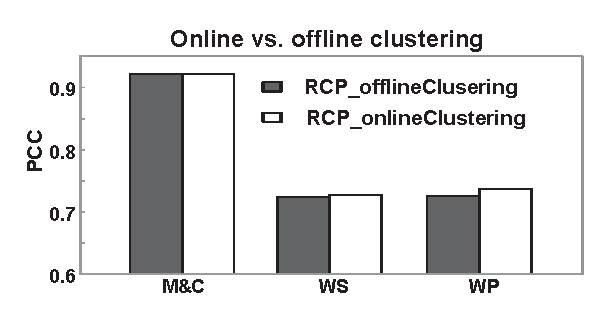
\includegraphics[width=\textwidth]{performanceCompareInOnlineAndOffline.eps}
% \caption{Performance of RCP with online/offline clustering}
% \label{fig:online-offiline}
%\end{minipage}
%\hfill
%\begin{minipage}[b]{0.32\textwidth}
% \includegraphics[width=\textwidth]{ComparisonOn300pairsAllMethods.eps}
% \caption{Performance comparison on WP}
% \label{fig:ComparisonOn300pairsAllMethods}
%\end{minipage}
%\hfill
%\begin{minipage}[b]{0.32\textwidth}
% \includegraphics[width=\textwidth]{Pearson-Performance-on-different-types-of-pairs.eps}
% \caption{Performance comparison on various types of pairs}
% \label{fig:Pearson-Performance-on-different-types-of-pairs}
%\end{minipage}
%\end{figure*}

\begin{figure}[!t]
 \centerline{
 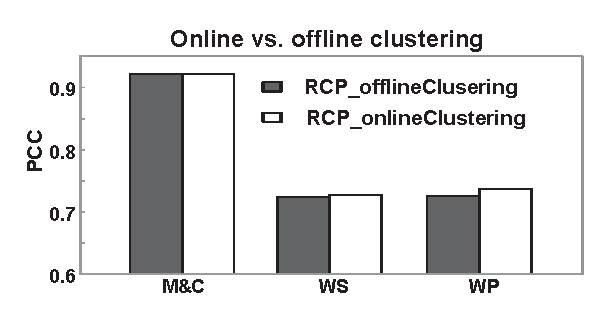
\includegraphics[width=0.8\columnwidth]{performanceCompareInOnlineAndOffline.eps}}
 \caption{Performance of RCP with online/offline clustering}
 \label{fig:online-offiline}
\end{figure}

\begin{figure}[!t]
 \centerline{
  \includegraphics[width=0.8\columnwidth]{ComparisonOn300pairsAllMethods.eps}}
 \caption{Performance comparison on WP}
 \label{fig:ComparisonOn300pairsAllMethods}
\end{figure}

\begin{figure}[!t]
 \centerline{
  \includegraphics[width=0.8\columnwidth]{Pearson-Performance-on-different-types-of-pairs.eps}}
 \caption{Performance comparison on various types of pairs}
 \label{fig:Pearson-Performance-on-different-types-of-pairs}
\end{figure}

\begin{figure*}[!t]
 \centerline{
 \includegraphics[width=1\textwidth]{curves-of-points-on-entity-pairs.eps}}
 \caption{Performance of our three approaches on entity pairs}
 \label{fig:online-entity-pairs}
\end{figure*}
\begin{figure*}[!t]
 \centerline{
 \includegraphics[width=1\textwidth]{curves-of-points-on-concept-entity-pairs.eps}}
 \caption{Performance of our three approaches on concept-entity pairs}
 \label{fig:online-concept-entity-pairs}
\end{figure*}

\begin{figure}[th]
 \centerline{
 \includegraphics[width=0.8\columnwidth]{entity-disambiguity.eps}}
 \caption{Performance of entity disambiguity in our approaches}
 \label{fig:entity-disambiguity}
\end{figure}
%\begin{figure*}[th]
%\begin{minipage}[bh]{0.32\textwidth}
% \centering
% 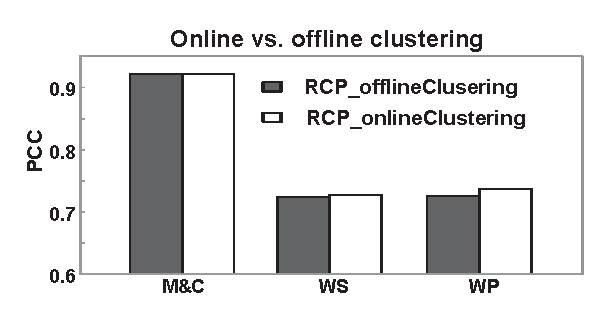
\includegraphics[width=\textwidth]{performanceCompareInOnlineAndOffline.eps}
% \caption{Performance of RCP with online/offline clustering}
% \label{fig:online-offiline}
%\end{minipage}
%%\hfill
%\hspace{2pt}
%\begin{minipage}[bh]{0.32\textwidth}
% \centering
% \includegraphics[width=\textwidth]{ComparisonOn300pairsAllMethods.eps}
% \caption{Performance comparison on WP}
% \label{fig:ComparisonOn300pairsAllMethods}
%\end{minipage}
%%\hfill
%\hspace{2pt}
%\begin{minipage}[bh]{0.32\textwidth}
% \centering
% \includegraphics[width=\textwidth]{Pearson-Performance-on-different-types-of-pairs.eps}
% \caption{Performance comparison on various types of pairs}
% \label{fig:Pearson-Performance-on-different-types-of-pairs}
%\end{minipage}
%\end{figure*}

\begin{figure}[th]
 \centerline{
 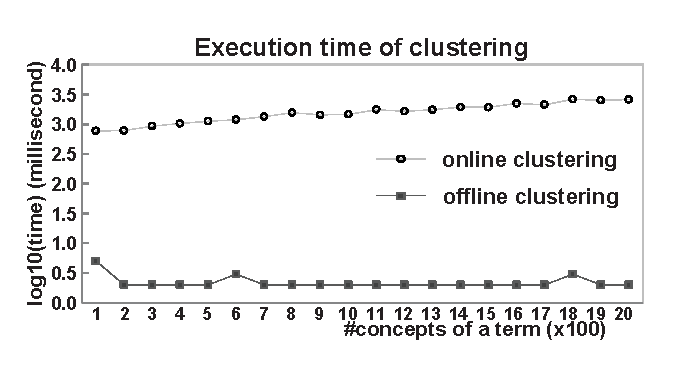
\includegraphics[width=0.4\textwidth]{TimeComparisonOfOfflineAndOnline.eps}}
 \caption{Execution time in online/offline clustering}
 \label{fig:TimeComparisonOfOfflineAndOnline}
\end{figure}

\begin{figure}[th]
 \centerline{
 \includegraphics[width=0.4\textwidth]{TimecomparisonOfDiffApproaches.eps}}
 \caption{Computation time in different approaches}
 \label{fig:TimecomparisonOfDiffApproaches}
\end{figure}

\begin{figure}[th]
 \centerline{
 \includegraphics[width=0.4\textwidth]{Time-Performance-on-different-types-of-pairs.eps}}
 \caption{Computation time on different types of pairs}
 \label{fig:Time-Performance-on-different-types-of-pairs}
\end{figure}

%\begin{figure*}[th]
%\begin{minipage}[bh]{0.32\textwidth}
% \centering
% 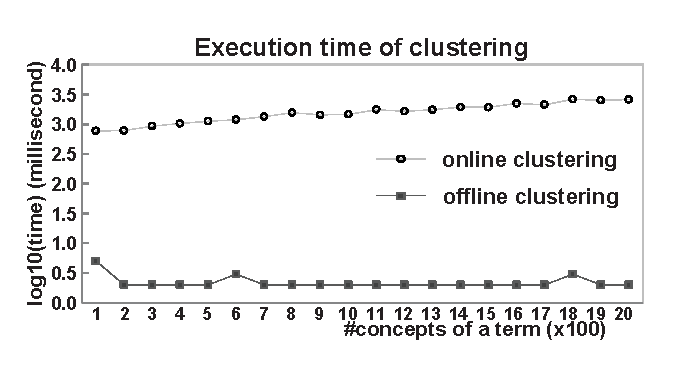
\includegraphics[width=\textwidth]{TimeComparisonOfOfflineAndOnline.eps}
% \caption{Execution time in online/offline clustering}
% \label{fig:TimeComparisonOfOfflineAndOnline}
%\end{minipage}
%\hspace{2pt}
%\begin{minipage}[bh]{0.32\textwidth}
% \centering
% \includegraphics[width=\textwidth]{TimecomparisonOfDiffApproaches.eps}
% \caption{Computation time in different approaches}
% \label{fig:TimecomparisonOfDiffApproaches}
%\end{minipage}
%\hspace{2pt}
%\begin{minipage}[bh]{0.32\textwidth}
% \centering
% \includegraphics[width=\textwidth]{Time-Performance-on-different-types-of-pairs.eps}
% \caption{Computation time on different types of pairs}
% \label{fig:Time-Performance-on-different-types-of-pairs}
%\end{minipage}
%\end{figure*}

%\begin{figure}[t]
% \centerline{
% \includegraphics[width=0.45\textwidth]{ComparisonOn300pairsAllMethods.eps}}
%\caption{Performance comparison on 300 pairs} \label{fig:ComparisonOn300pairsAllMethods}
%\end{figure}
%
%\begin{figure}[t]
% \centerline{
% \includegraphics[width=0.5\textwidth]{Pearson-Performance-on-different-types-of-pairs.eps}}
%\caption{Performance comparison on different types of pairs} \label{fig:Pearson-Performance-on-different-types-of-pairs}
%\end{figure}

%\begin{table}[th]
%\centering
%\caption{Examples of Computation Results in Our RCP approach}
%\label{tab:exampleOfOurResults}
%{
%\begin{tabular}{|l|c|}\hline
%pair & similarity score\\\hline
%\multicolumn{2}{|c|}{on M\&C data set}\\\hline
%\pair{bird}{cock} &    0.824\\\hline
%\pair{boy}{lad}    &0.800\\\hline
%\pair{coast}{shore}    &0.800\\\hline
%\pair{bird}{crane} &0.564\\\hline
%\pair{crane}{implement}    &0.294\\\hline
%\pair{monk}{oracle}    &0.002\\\hline
%\pair{journey}{car}    &0.001\\\hline
%\pair{lad}{wizard} &0.000\\\hline
%\multicolumn{2}{|c|}{on WS data set}   \\\hline
%\pair{tiger}{jaguar}   &0.979\\\hline
%\pair{professor}{doctor}   &0.930\\\hline
%\pair{vodka}{brandy}   &0.929\\\hline
%\pair{journey}{voyage} &0.800\\\hline
%\pair{travel}{activity}    &0.532\\\hline
%\pair{consumer}{energy}    &0.518\\\hline
%\pair{man}{governor}   &0.506\\\hline
%\pair{precedent}{information}  &0.011\\\hline
%\multicolumn{2}{|c|}{on WP data set}       \\\hline
%\pair{caged animal}{game animal}   &0.996\\\hline
%\pair{bank}{citibank}  &0.966\\\hline
%\pair{business}{restaurant}    &0.938\\\hline
%\pair{date}{asian pear}    &0.711\\\hline
%\pair{range}{food processor}   &0.689\\\hline
%\pair{climacteric fruit}{vegetable juice}  &0.226\\\hline
%\pair{apple}{garlic}   &0.019\\\hline
%\pair{music}{lunch}    &0.012\\\hline
%\end{tabular}
%}
%\end{table}

\begin{table}[th]
\centering \caption{Example Pairs and Their Semantic Similarity Scores Computed by RCP Approach
%{\color{red}(Human Ratings are
%normalized into [0,1] in this table)}
} \label{tab:exampleOfOurResults} {
\small
\begin{tabular}{|l|c|c|}\hline
&Human& Similarity\\
Pair &Rating& Score\\\hline \multicolumn{3}{|c|}{From M\&C Data Set}\\\hline \pair{furnace}{stove}   &0.778&0.950\\\hline \pair{bird}{cock}
&0.763&0.824\\\hline \pair{boy}{lad} &0.940&0.800\\\hline \pair{coast}{shore} &0.925&0.800\\\hline \pair{bird}{crane} &0.743 &0.564\\\hline
\pair{lobster}{food}&0.223 &0.525\\\hline \pair{crane}{implement}&0.420 &0.294\\\hline \pair{monk}{oracle}&0.275 &0.002\\\hline
\pair{journey}{car} &0.290&0.001\\\hline \pair{chord}{smile} &0.033&0.000\\\hline \multicolumn{3}{|c|}{From WS Data Set}  \\\hline
\pair{tiger}{jaguar} &0.800&0.979\\\hline \pair{professor}{doctor} &0.662&0.930\\\hline \pair{vodka}{brandy} &0.813 &0.929\\\hline
\pair{journey}{voyage} &0.929&0.800\\\hline \pair{travel}{activity} &0.500&0.532\\\hline \pair{consumer}{energy} &0.475&0.518\\\hline
\pair{man}{governor} &0.525&0.506\\\hline \pair{reason}{hypertension} &0.231&0.036\\\hline \pair{precedent}{information} &0.385  &0.011\\\hline
\pair{lobster}{wine} &0.570   & 0.000\\\hline
\multicolumn{3}{|c|}{From WP Data Set}
\\\hline \pair{caged~animal}{game~animal} &0.850&0.996\\\hline \pair{business}{restaurant} &0.550&0.938\\\hline \pair{shell}{exxon~mobil~corp.}
&0.850&0.814\\\hline \pair{animal}{poodle} &0.800  &0.720\\\hline \pair{date}{asian~pear} &0.500&0.711\\\hline \pair{range}{food~processor}
&0.750&0.689\\\hline \pair{climacteric~fruit}{vegetable~juice} &0.600  &0.226\\\hline \pair{music}{lunch} &0.100&0.012\\\hline
\pair{banana}{beef} &0.350&0.007\\\hline \pair{apple}{ipad}&0.200  &0.006\\\hline
\end{tabular}
}
\end{table}

\subsection{Efficiency}
In this subsection, we aim to observe the efficiency of our approaches.
Figure~\ref{fig:TimeComparisonOfOfflineAndOnline} compares the execution time between online clustering and offline clustering in our refined
approach. Offline clustering, with only a fraction of the cost, is a clear winner.
%Offline clustering clearly saves a lot of time in
%Figure~\ref{fig:TimeComparisonOfOfflineAndOnline}.
%compares the execution time between online clustering and offline clustering in our refined
%approach. Offline clustering, with only a fraction of the cost, is a clear winner.
%where the execution time of online clustering indicates the time cost of clustering the given concepts of the term, while the execution time of offline clustering indicates the time cost of finding clusters according to the clustering results in $\Gamma_{cluster}$. From the experimental results, we can see that the time complexity of online clustering is approximately in a direct proportion to the number of clustering objects (namely the count of concepts the given term belongs to), while the time complexity of offline clustering is almost a const value. More precisely, as the number of the concepts increases from 100 from 2000, the execution time of online clustering varies from 770 milliseconds to 2582 milliseconds while the execution time of offline clustering is always no more than 5 milliseconds. These data reveal that offline-clustering is more efficient, which is conducive to improve the efficiency in the calculation of the semantic similarity between terms.

Figure~\ref{fig:TimecomparisonOfDiffApproaches} reports the average computation time on a pair of terms in our approaches compared to the other
competitors. On average, RCP takes 65 milliseconds to compute the similarity of a pair, which is on par with most of the earlier methods using
information content and WordNet. String-based methods are faster for an obvious reason: they need not collect any context or model the context.
%Two methods are significantly slower than RCP and the crowd.
Hir is slow because it considers the lexical chain in the taxonomy in the
calculation of semantic similarity between terms.
%It requires traveling the
%taxonomy tree to find the hypernym and hyponym of terms. %\KZ{But why this slow??}
Bol takes about 60 times longer than RCP because
it requires extracting lexico-syntactic patterns from snippets online.
%which is very time consuming.
%It is slower than the string-based method of Hun and Tra.
%This is because the string-based methods needn't collecting any
%contexts of terms and modeling the contexts.
%However, as compared to the path-based and lexical chain-based methods,
%it is faster than the Hir and Do methods, which is less than
%1/2 of their time cost, while it is slower than the Rad method
%by 14 milliseconds.
%while Rad only use the minimum path length.
%The former especially the Hir method requires traveling the
%taxnomy tree to find the hypernym and hyponym information of terms.
%As compared to the IC-based methods, it is comparable to
%the Res, Jcn, Lin and San methods. For these IC-based methods,
%all IC values of terms involved in WordNet are prepared well, the only time consumption lies in the traveling of ontology tree. As compared to the glossed-based method Ban and the PageRank-based method Agi, it only consumes 1/2 of their time cost. This is because Ban needs to compare all glosses of the given term, and Agi needs to compute the probability of a random-walk initiated in the target word to reach any synset following the relations in WordNet.
%As compared to our Basic approach, because RCP needs clustering all concept contexts, which consumes more time. It is hence slower than Basic by 14 milliseconds. However, it is faster than RC by 100 milliseconds. This is because RC produces much more small sized clusters than RCP, and it needs comparing each pair of clusters to get the maximum one while RCP only maintains large sized clusters by cluster pruning. Though cluster pruning introduces the additional time consumption, it is much lower than the total time consumption in the comparing each pair of clusters in RC.

Figure \ref{fig:Time-Performance-on-different-types-of-pairs} shows
the average computation time on different types of pairs
using our approaches.
%From the experimental results, we observe the following.
%First, our three approaches can get the semantic similarity of a
%concept pair in 24 milliseconds.
%Second, on the entity pair and the concept-entity pair,
%RCP is comparable to Basic.
%Both approaches demand a lighter time overhead compared to RC.
%More specifically, Basic and RCP averagely consume 47 milliseconds
%and 125 milliseconds on an entity pair and a concept-entity pair
%respectively while RC consumes 216 milliseconds and 252 milliseconds
%respectively.
RCP costs less than half the time of RC due to the pruning.
%\KZ{Is this correct?}
Computing similarity between
concept-entity pairs is more expensive
because in order to catch the concept-entity pairs
with potentially transitive isA relationships, e.g., ``animal'' and
``puppy'' (with ``dog'' being the child of ``animal'' and parent
of ``puppy''), we iteratively check the relations between
every top ancestor concepts of an entity term and
the concept term in RCP. %\KZ{Check if the above is correct.}
%This imposes the computation time compared to that on
%the entity pair and concept pair.
%?gIn an overall considering,
%?gthe computation time on a pair is averagely 51 milliseconds,
%?g164 milliseconds and 66 milliseconds respectively in our
%?gBasic, RC and RCP approaches.

%\begin{table}[!h]
%\centering
%\caption{Case Study of Refined Approach}
%\label{tab:examples}{\scriptsize
%\begin{tabular}{|c|c|c|c|}\hline
% & &Basic & Refined \\
%termA & termB   & in Eq.~\ref{eq:cosine} & in Eq.~\ref{eq:clusterCosine}\\\hline
%\textbf{Apple} &Pear    &0.916  &\textbf{0.999}\\
%\textbf{Apple}&Microsoft        &\textbf{0.378} &\textbf{0.994}\\
%\textbf{Orange}&Pear    &0.715  &\textbf{0.845}\\
%\textbf{Orange}&Red     &\textbf{0.491} &\textbf{0.982}\\
%Microsoft&\textbf{GE}   &0.620  &\textbf{0.982}\\
%Music&Lunch     &0.012  &\textbf{0.884}\\
%Company&Microsoft       &0.930  &\textbf{0.934}\\
%Asia~country &Developing~country        &0.852  &0.852\\
%Country&Company &0      &0\\
%\hline
%\end{tabular}}
%\end{table}

%\begin{figure*}[t]
% \centerline{
% \includegraphics[width=0.9\textwidth]{Performance-on-different-types-of-pairs.eps}}
%\caption{Performance comparison in our approaches on different types of pairs} \label{fig:Performance-on-different-types-of-pairs}
%\end{figure*}

\section{Related Work}
\label{sec:related}

Contrary to the semantic relatedness which represents the more general relationships such as part-whole and the co-occurrence, semantic
similarity measures the degree of taxonomic likeness between concepts and considers relations such as hyperonymy and synonymy. In this section,
we only discuss previous work on semantic similarity, while most of them can be adapted or generalized to deal with semantic relatedness. To
compute the semantic similarity between terms, existing efforts mainly
follow two approaches: The first approach calculates the semantic
similarity based on some distance in a preexisting thesauri, taxonomy or encyclopedia, such as WordNet. The second approach computes similarity
by the terms' context in large text corpora (such as the search snippets and web documents) and such similarities are derived from
distributional properties of words or n-grams in the corpora.
%{\color{red} Clearly, all of term co-occurrence based methods also
%belong to the corpus-based approach.}

\subsection{Knowledge-based Approach}

Most methods in this direction use a taxonomy such as WordNet, which is
a tree hierarchy, as the knowledge base to compute
the similarity between terms.
%One is the concept likeness based approach regarding the relationships in
%WordNet and the other is the the graph-based learning approach built on
%the isA-relationship structure of WordNet.
The most straightforward way to calculating similarity between two
terms on the WordNet is to find the length of the shortest path
connecting the two terms in the taxonomy graph\cite{Rada:1989}.
This path-length based approach is very simple, but has a low accuracy
because: i) it relies on the notion that all links in the taxonomy represent
a uniform distance; ii) it ignores the amount of information hidden in the concept nodes.

More advanced approaches \cite{Resnik:1995, Jiang:1997, Lin:1998, Seco:2004, Snchez:2011} compute the similarity between $t_1$ and $t_2$ by the
information content of these terms with respect to the taxonomy structure. The pioneer work by Resnik \cite{Resnik:1995} suggests that the
similarity measure is the information content of the least common ancestor node of the two terms in the taxonomy tree.
%between two concepts $c_{1}$ and $c_{2}$ in the taxonomy as the maximum of the information content of all concepts \emph{C} that
%subsume both $c_{1}$ and $c_{2}$, and then it takes the maximum of the similarity between any concepts that the terms belong to as the final
%semantic similarity.
To compute the information content of a term, it requires a large text corpus
to obtain the occurrences of the term.
A limitation of this method is that the similarities between all children of
a concept are identical, regardless of their individual information content.
The most recent information content based approach \cite{Snchez:2011} calculates
the information content of term $t$ by the ratio of
the number of hypernyms of $t$ divided by the number of all descendants of $t$ in WordNet. 
%Pedersen etc. adapted the above measures to the SNOMED-$CT^(R)$ ontology of medical concepts. Meanwhile, they also derived a context vector measure based on medical corpora that can be used as a measure of semantic relatedness.
Some of the above measures have been adapted to the biomedical field by incorporating domain information extracted from clinical data or from medical ontologies (such as MeSH or SNOMED-$CT^{(R)}$)\cite{Pedersen:2007, Batet:2011}.
 
%This method yields a Pearson correlation coefficient of up to
%0.87 on the M\&C benchmark database.

%The first work applying information theory to semantic similarity
%computation was proposed by Resnik \cite{Resnik:1995}. It states concept
%similarity depends on the amount of shared information
%between two concepts. That is, given two concepts $c_1$ and $c_2$, the algorithm first finds the most specific common ancestor subsuming both
%concepts (denoted as the Least Common Subsumer: LCS) by exploiting a background ontology. Secondly, it uses the information theoretic evaluation
%function to compute the IC (Information Context) value of LCS, and it computes the $IC$ of a concept by $-log(p(c))$, where $p(c)$ indicates the
%probability of encountering \emph{c} or any of its taxonomical hyponyms in the given corpus. The popular corpus include the SemCor texts distributed
%with WordNet 3.0, Brown corpus and British National Corpus. In this algorithm, there is a problem that any pair of concepts with the same LCS will
%result in exactly the same semantic similarity. Thus, to tackle this problem, researchers have extended the Resnik's work by considering the IC of
%each of the evaluated concepts. For example, Jiang and Conrath proposed to quantify the length of the taxonomical links as the difference between
%the IC of a concept and its subsumer\cite{Jiang:1997}. Instead of subtracting the IC of their LCS from the sum of the
%IC of each concept as the similarity between two concepts, Lin adopted the ratio between the amount of the IC of their LCS and the sum of the IC of
%each concept to measure their similarity.
%
%In the analysis of corpora-based IC algorithms mentioned above, researchers found that to accurately compute the information therapy, the contents of corpora should be adequate regarding the ontology scope and big enough. However, large and general purpose corpora such as Brown corpus and British National Corpus may be only suitable for WordNet. Therefore, some authors proposed computing IC from an ontology in an
%intrinsic manner\cite{Seco:2004} without the corpus. Comparing corpora-based IC computation models, the intrinsic IC-based models take a function of the
%number of hyponyms in a taxonomy as the appearance probability of a concept (and the amount of information it provides). For example, Seco et al. first proposed to compute the base IC calculations on the number
%of concept hyponyms \cite{Seco:2004}. S$\acute{a}$nchez et. al. proposed an advanced intrinsic IC computation algorithm \cite{Snchez:2011}, which combines the information of the number of leaves in all hyponyms of the concept $c$ and the number of taxonomical subsumers that the concept $c$ belongs to.

%Considering the graph-based learning approach built on the ontology structure of
%WordNet, the representative works are below.
Other researchers attempted to apply graph learning algorithms
on term similarity computation.
Given two terms $t_1$ and $t_2$, Alvarez and Lim \cite{Alvarez:2007}
build a rooted weighted graph called $Gsim$,
using the terms hypernyms, other relations, and descriptive
glosses from WordNet, and then calculate the similarity score
by selecting the minimal distance between any two hypernyms $c_1$ and
$c_2$ of $t_1$ and $t_2$ respectively, by random walk.
%The authors claimed that this method achieves
%a pearson correlation coefficient of 0.913
%on the M\&C benchmark data set\cite{Miller:1998}.
Agirre et. al. subsequently proposed a WordNet-based personalized PageRank
algorithm \cite{Soroa:2009, Agirre:2010}. It first computes
the personalized PageRank of each word and aggregates into
a probability distribution for each synset. Similarity is then defined by
the cosine between two distributions.
%any two discrete probability distributions are by
%encoding them as vectors and computing the cosine similarity between the vectors.
%In addition, authors trained a SVM to combine three basic
%methods including bag-of-words, context-window-based method and the WN30g-based method \cite{Agirre:2009}. In this case, the highest pearson
%correlation coefficient is up to 0.93 on the M\&C benchmark data set.

The above knowledge based approaches depend heavily
on the completeness of the underlying taxonomy and
the external corpora.
%To provide reliable results at a conceptual level, it requires the
%knowledge source must be as complete as possible, namely,
%it should include most of the specializations of each concept covered in the corpus.
However, the popular taxonomy like WordNet does not have the adequate coverage
as it cannot keep up with the development of new terms and phrases everyday.
%especially for the Web data. Meanwhile, to avoid data sparseness in
%the information content computation, it requires contents of corpora should
%be adequate and big enough regarding the ontology scope.
%Similarly, popular corpora such as the SemCor\cite{semcor} texts
%distributed with WordNet 3.0, Brown corpus\cite{Brown} or
%British National Corpus\cite{BNC} are mostly designed for WordNet,
%and have limited coverage on terms beyond that.

The framework proposed in this paper is also knowledge based, but is
more scalable and effective,
because i) the knowledge we use was acquired from the entire Web; and
ii) the clustering algorithm detects the senses of the input terms
and the max-max similarity function effectively picks the senses that are most
suitable given the pair of terms. The above methods cannot be easily adapted
to use Probase because it is a general network, not a tree structure.

\subsection{Corpus-based Approach}

%Regarding the distributional context based similarity evaluation approaches, main works are below.
%Sahami et al. measured semantic similarity
%between two queries using search snippets\cite{Sahami:2006}. For each query, the proposed approach first collects snippets from a search engine
%and represents each snippet as a TF-IDF weighted term vector, and then it defines the semantic similarity between two queries by the inner product
%between the corresponding centroid vectors.
In this space, Chen et. al. proposed a double-checking model
using text snippets returned by a Web search engine
to compute semantic similarity between words \cite{Chen:2006}.
The proposed method uses the occurrences of terms $X$ and $Y$
in their search snippets to evaluate the semantic similarity.
Recently, Bollegala et.al. proposed a new measure using
page counts and snippets from Web search \cite{Bollegala:2011}.
%To compute the similarity between $X$ and $Y$,
%it first collects the snippets from a web search engine by
%querying ``\emph{X} AND \emph{Y}'', and then extracts lexical patterns that combine \emph{X} and \emph{Y} from snippets. Then it uses
%frequencies of 200 lexical patterns in snippets and four co-occurrence measures: Dice coefficient, overlap coefficient, Jaccard coefficient and
%pointwise mutual information to create the feature vectors. Finally, it trains a two-class support vector machine using automatically selected
%synonymous and non-synonymous word pairs from WordNet. This method reports a Pearson correlation coefficient of 0.837 with Miller-Charles
%ratings.
%However, the above methods heavily depends on the search engine's
%ranking algorithms.
The search engine based methods are more time-consuming because
i) snippets and search results must be obtained online;
ii) it requires parsing of the returned text by the patterns.

Radinsky et. al. proposed
a new model, Temporal Semantic Analysis (TSA)
\cite{Kira:2011}, which captures the temporal information of corpus.
TSA uses a more refined representation, where each concept is no
longer scalar, but is instead represented as time series over a
corpus of temporally-ordered documents. This method can improve the
pearson correlation coefficient, but it requires massive historical data.
%which leads to more time-consuming in the handling of texts.

Most corpus based methods are more suitable for the semantic
relatedness not for the semantic similarity because they
make heavy use of the co-occurrence context in the representation
of terms or in similarity functions.
%%% Local Variables:
%%% mode: latex
%%% TeX-master: "main"
%%% End:

\section{Conclusions}
\label{sec:conclude}

Accurately computing semantic similarity between terms is 
a challenging task in the applications of text analytics and 
text understanding.  In this paper, we
presented a lightweight, effective approach for semantic similarity 
between terms with any multi-word expression. 
Our approach first utilizes the isA relationships extracted 
from the Web data as the semantic contexts of the terms. 
Second, it installs clustering on the collected contexts 
to find potential senses of the terms, and then it compares 
the cluster-based contexts to get the semantic similarity between terms. 
When compared to the state-of-the-art semantic similarity computation
methods and the basic algorithm, 
our clustering-based approach has a higher pearson 
correlation coefficient on benchmark data sets with word pairs 
and MWE pairs. Meanwhile, it is more applicable to the 
large scale data sets due to its lower time cost in the 
calculation of semantic similarity between terms.


\section{Acknowledgments}
This work is supported in part by National 863 Program of China under grant 2012AA011005, the National 973 Program of China under grant
2013CB329604, the Natural Science Foundation of China under grants (61100050, 61273292, 61229301, 61070131, 61273297), the Postdoctoral Science
Foundation of Hefei University of Technology under grant 2013HGBH0025, MOE New Faculty under grant 201100731- 20023, and the US National Science Foundation (NSF) under grant
CCF-0905337.
%\input{ThreeExamples}
%
% The following two commands are all you need in the
% initial runs of your .tex file to
% produce the bibliography for the citations in your paper.
\bibliographystyle{abbrv}
\bibliography{similarity}  % sigproc.bib is the name of the Bibliography in this case
% You must have a proper ".bib" file
%  and remember to run:
% latex bibtex latex latex
% to resolve all references
%
% ACM needs 'a single self-contained file'!
%
%APPENDICES are optional
%\balancecolumns
%\appendix
%Appendix A
%\balancecolumns
% That's all folks!
%\end{multicols}
\end{document}
